\section{Volvo Cars architecture framework}\label{sec:VCGAF}

The starting point for defining an architecture framework is to start from the identification of established stakeholders within the domain of the framework. Stakeholders may be individuals, teams,
organizations or classes (of individuals, teams or organizations), while concerns may be fine-grained or very broad in scope~\cite{Emery-Hilliard:2009}. 

%Table \ref{tab:stakeholders} describes the main actors in the challenging scenarios.
% \todo[inline]{elaborate and describe. Also: Include other stakeholders such as customer, driver, ...}

%A suitable electrical architecture needs to take into account the specific needs of each of these stakeholders. 
%In the next section, we will discuss \emph{challenging scenarios} that explore how these stakeholders will interact with the electrical system, its architecture, and its development.

\begin{table}[htb]
\scriptsize
\caption{Overview of Stakeholders}
\label{tab:stakeholders}
\begin{tabular}{rv{0.14\textwidth}v{0.2\textwidth}v{0.26\textwidth}v{0.2\textwidth}}
\toprule
& \textbf{Stakeholder} &	\textbf{Group} & \textbf{Comment} & \textbf{Synonyms} \tabularnewline
\midrule
$\bullet$& Passengers & end-user	\tabularnewline
$\bullet$& Drivers & end-user		\tabularnewline
$\bullet$& Customers & customer & Purchaser of a car or related service & \tabularnewline
$\bullet$& Product planner & customer & Acquirer of electrical system		\tabularnewline
$\bullet$& Purchaser & customer & Purchasers of electrical system		\tabularnewline
$\bullet$& Line managers & management & Has scheduling responsibility, long term quality responsibility, includes group, department	\tabularnewline
$\bullet$& Project managers & management & Owns budget for development	\tabularnewline
$\bullet$& System architects & developers of electrical system & 	\tabularnewline
$\bullet$& Functional developers & developers of electrical system & Owns functional and non-functional aspects & function owner; function realizer; function developer, function realizer, system developer\tabularnewline
$\bullet$& Component developers & developers of electrical system		\tabularnewline
$\bullet$& SW supplier (internal/external) & developers of electrical system	& Can be internal or external from the perspective of the OEM.	\tabularnewline
$\bullet$& HW supplier (internal/external) & developers of electrical system	& Can be internal or external from the perspective of the OEM.	\tabularnewline
%SW supplier (external & developers of electrical system		\tabularnewline
%HW supplier (external) & developers of electrical system		\tabularnewline
$\bullet$& Testers & developers of electrical system		\tabularnewline
$\bullet$& Attribute Owners & developers of electrical system & Owns non-functional attributes like performance	\tabularnewline
$\bullet$& Tool Engineers & developers of electrical system & Specifically testing tools, including design tools (e.g. for requirements)	\tabularnewline
$\bullet$& Calibrators & developers of electrical system & \tabularnewline
$\bullet$& Diagnostic method engineers & maintainers of electrical system		\tabularnewline
$\bullet$& Workshop Personnel & maintainers of electrical system		\tabularnewline
$\bullet$& Fault Tracing Specialists & maintainers of electrical system		\tabularnewline
$\bullet$& Technical Specialist &  specialists &	Support developers and maintainers on specific topics \tabularnewline
\bottomrule
\end{tabular}
\end{table}

Table~\ref{tab:stakeholders} describes the main stakeholders we have identified; they fall into five major groups: 

\begin{itemize}
\item \emph{End-users} of the electrical system, like drivers and passengers.
\item \emph{Customers} stakeholders, such as paying customers of products and services that depend on the electrical system (i.e. the car) and product planners, who acquire the electrical system as part of the overall product.
\item \emph{Management} with responsibility for scheduling, long term quality, groups, departments, and budget.
\item \emph{Developers of the electrical system}  include engineers throughout the value chain that create the electrical system, its architecture, and the necessary tools as well as that test and integrate the various components. 
\item \emph{Maintainers of the electrical system} who interact with the electrical system throughout its lifetime. 
\end{itemize}


Then the identified stakeholders motivate the set of concerns on which the architecture framework will focus.
This will help the consumer of the architecture framework and of the views and connected modeling tools to understand why
they are modeling and when they are done.
In order to define the stakeholders concerns we identified a set of challenging scenarios through a number of workshops for elicitation and validation. 
Figure~\ref{fig:challenging-scenarios} gives an overview of the scenarios that are strongly connected to the viewpoints we will detail in this paper. These scenarios are described in the following items.
\magnus{Rogardt and I made a draft picture with the use cases from WP3 added.
Color, exact naming, bubble placement etc., TDB.
Do you think this is a workable way forward?}\patrizio{Magnus, might you please change the figure according to the new text I wrote? I don't have the source files.}

\begin{figure}[htb]
\begin{center}
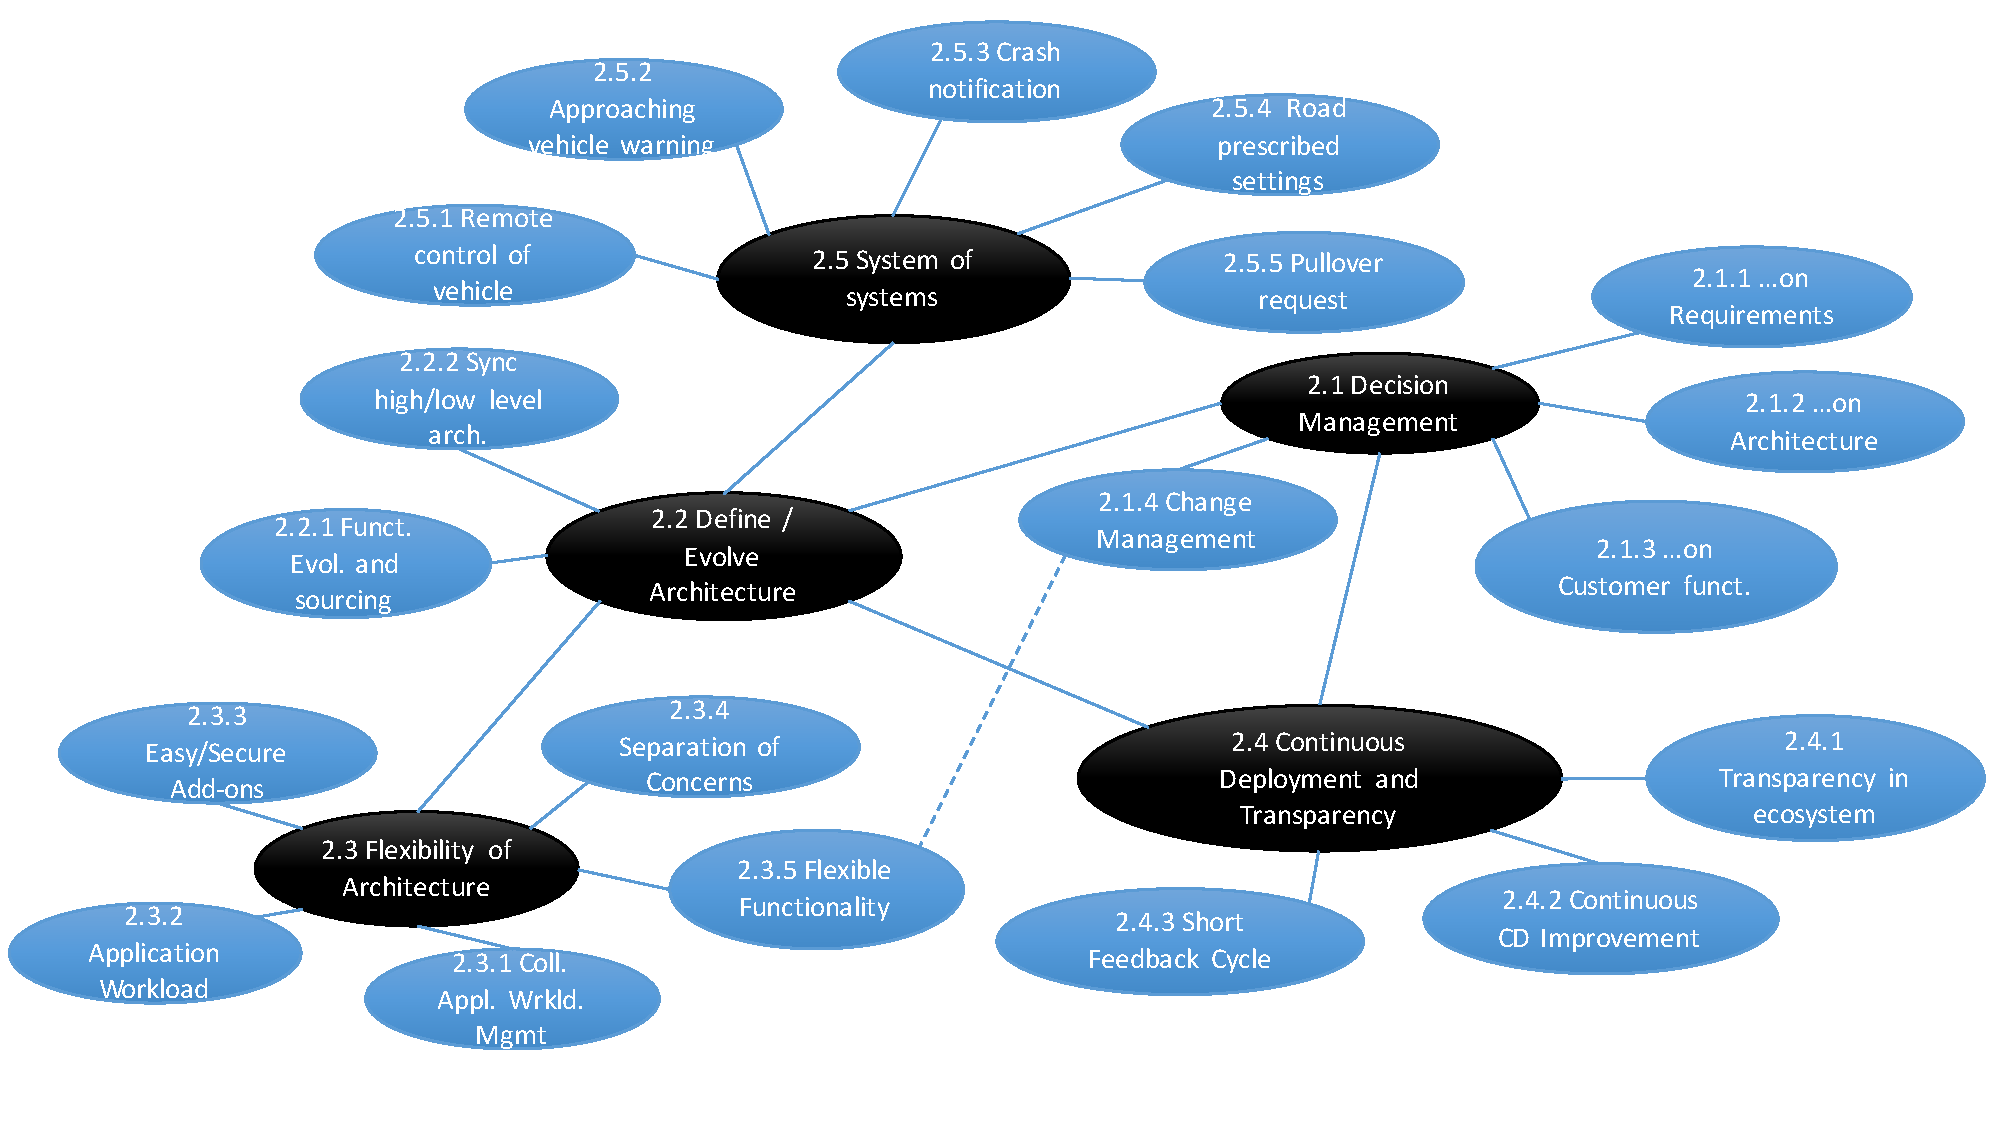
\includegraphics[width=\textwidth]{figures/WasaUseCaseDiagram} 
\caption{Overview of challenging scenarios}
\label{fig:challenging-scenarios}
\end{center}
\end{figure}


\begin{itemize}
\item Scenario 2.1 {\bf decision management } aims at exploring how to make, communicate, and manage decisions. 

\begin{quote}
{User Story:} \emph{``As a member of the development ecosystem I would like to have a clear understanding on how to take decisions and how to communicate them.''}
\end{quote}


Interesting sub-scenarios include decisions about:

\begin{itemize}
\item  {\em Requirements (2.1.1)}: When decisions on requirements are made too early, it will lead to unnecessary changes.

%\textbf{Trigger:} Requirement needs to be refined so that others can continue working.

\begin{quote}
{User Story:} 
\emph{``As a component responsible, I need to write a requirement. 
Currently, I am forced to write the requirement in a certain document or certain structure. 
This determines whether the requirement refers to a hw or sw component, whether it will be implemented in-house or by an external supplier. 
Often, it is too early to make such decisions and changes are necessary later, when more information becomes available. 
I do not feel comfortable to make this decision so early.''}
\end{quote}

\item {\em Architecture (2.1.2)}: Architectural decision making involves making the right decision, communicating it, ensuring that it is followed, and changing it when needed. 

%\textbf{Trigger:}  Architectural decision required (it is beneficial and possible). 

\begin{quote}
{User Story:} 
\emph{``As an architect} (one of \{system architect; functional developer; low level architect\})\emph{, I need to make the right decision at the right moment (i.e. when it is useful to make the decision and when the necessary information is available).  
I need to make this decision on the right level. 
I need to be introvert to make the best possible decision on the available data and extrovert to communicate it.''}
\end{quote}

\item {\em Customer functions (2.1.3)}:  Electrical architecture is guiding realization of customer functions, but it is not obvious how the architecture support customer functions (with respect to tracing and methodology).

%\textbf{Trigger:}  Decision about customer function required. 

\begin{quote}
{User Story:} 
\emph{``As a product manager, I want to be supported by the electrical architecture in making decisions about customer functions. Based on a wishlist from the Market Analysis Department, I engage in a dialog with the departments that design the system. 
For this task, I wish for support from an electrical architecture that not only takes into account non-functional aspects, but also the nature of customer functions (which changes over time).''}
\end{quote}

\item {\em Change management (2.1.4)}: Good flexibility of the architecture allows us to continuously remove assumptions and do changes even late in the process. 
However, in a weak electrical architecture, such changes will impact the stability of the electrical system because of technical dependencies. 

\begin{quote}
{User Story:} 
\emph{``As a product planner I want to have a flexible Change Management process, allowing me to change or add functions late in the process, often with the goal of removing assumptions. 
This includes for example defining and changing the allocation of Functions to ECU late in the process.''}
\end{quote}
\end{itemize}
 
 
\item Scenario 2.2 {\bf define/evolve architecture} explores aspects of long-time evolution of the electrical architecture.
This includes:

\begin{itemize} 
\item {\em The impact of long-term sourcing decision on the logical architecture (2.2.1)}: Long term sourcing contracts allow to optimize production cost, but constraint evolution of the architecture. 
\begin{quote}
{User Story:} 
\emph{``As a Function Developer I want to optimise the evolution of functions without considering sourcing agreements. 
Today I have to discuss with the product planner about the plan for a function two years or more in advance to reflect on existing contracts, e.g. when related nodes are sourced for different time intervals. Problem: Sourcing needs make physical layout dominate logical decisions.''}
\end{quote}

%Architectural frameworks such as AUTOSAR can support functional evolution on component level, but addressing this scenario would also require more  thinking on how to support moving around functions on high level architecture.

\item {\em The danger of architecture and design  evolving in different directions (2.2.2)}: If not actively managed,  architecture and design diverge over time. 
The architecture is then perceived as outdated and not useful, thus it looses its ability to guide design decisions and implementation.

\begin{quote}
{User Story:} 
\emph{``As a system architect or function developer I want a stringent correlation between architecture and design. Otherwise, one or the other is wrong. ''}
\end{quote}
\end{itemize}

\item Scenario 2.3 {\bf flexibility of architecture} addresses different scenarios that emphasize flexibility of the electrical architecture, both on a technical and on a process level. On a technical level, more capacity in the ECUs allows to add functionality late. 
On a process level, the available resources need to be managed across several contributing partners.
This includes:

\begin{itemize}
\item {\em application workload management from a process perspective (2.3.1)}: 
\begin{quote}
{User Story:} 
\emph{``As a functional developer, I want to be flexible when it comes to application workload. 
Suppliers should be able to acquire and return resources dynamically throughout the lifecycle. ''}
\end{quote}
\item {\em application workload management from a technical perspective (2.3.2)}: higher capacity of ECUs and Buses will facilitate late or even very late updates (i.e. when the vehicle is on the street), because new functionality could use more resources.
This flexibility comes at a cost and it is not trivial to understand where the break-even point is.

\begin{quote}
{User Story:} 
\emph{``As a system architect I want to balance capacity of ECUs and Buses against cost.''}
\end{quote}

\item {\em easy and secure add-ons (2.3.3)}: being able to add new functions in a secure and easy way would allow to detach software development to some extend from the development cycle. 
During the development of a car, an OEM could focus on the critical basic functionality. 
Convenience features as well as more advanced connected features could be added independent from the start of production.
This would allow to develop more continuously and should decrease the peak of trouble reports before critical deadlines observed earlier~\cite{modelsward13}.

\begin{quote}
{User Story:} 
\emph{``As a  functional developer I want to be able to add new functions (very) late. Such add-ons could originate from third parties and should be added even after the vehicle has been put into use. ''}
\end{quote}

\item {\em separation of concerns (2.3.4)}: 
\begin{quote}
{User Story:} 
\emph{``As a system architect, I want to balance separation of concerns on two levels: between domains (e.g. safety vs. infotainment) and levels of abstractions (e.g. architecture vision vs architecture implementation).''}
\end{quote}

\item {\em flexible functionality (2.3.5)}:
\begin{quote}
{User Story:} 
\emph{``As a functional developer, I want to be flexible about the functions that are running in the car and allow for very late deployment. ''}
\end{quote}
\end{itemize}
 
\item Scenario 2.4 {\bf continuous deployment and transparency} includes:

\begin{itemize}
\item {\em the need for openness and transparent information through out the different value chains in the automotive ecosystem (2.4.1)}: Good transparency in the value chain supports flexibility, since all partners can take appropriate action to reach a (changing) goal quickly. 
The \emph{cone of uncertainty} is a good example for this~\cite{cone-of-uncertainty,cone-of-uncertainty2}: In the beginning of a project, not much data is available and decisions are very uncertain. 
As the project proceeds, assumptions are removed and uncertainty is reduced, but as  a consequence, it becomes harder to make decisions that change a lot. 
Good transparency can help to reduce the uncertainty quicker and can allow to decide fast in order to learn fast.
m
\begin{quote}
{User Story:} 
\emph{``As any developer of the electrical system (internal or external), I want to have access to relevant decision, to the status of relevant assumptions, and knowledge generated during the development. 
This allows me to participate in the fast learning throughout the value chain and enables me to be effective and flexible in my work.''}
\end{quote}

\item {\em the need for using this information to continuously improve an continuous integration, delivery, and deployment flow (2.4.2)}: 
Cross-organizational continuous integration, delivery, and deployment facilitates fast feedback and rich learning.
This learning should also help to improve the interaction of organizations and the integration flow between them.

Have a culture of continuous improvement between VCC and partners	Apply Continuous Deployment to the CD tool chain

\begin{quote}
{User Story:} 
\emph{``As a Project Manager, I want to have a culture of continuous improvement within the OEM and with partners in the value-chain. As any developer of the electrical system (internal and external) I want to benefit from and take responsibility in improving the continuous delivery flow.''}
\end{quote}

\item {\em the need for establishing short feedback cycles (2.4.3)}: While developing new functionality, basic software, and hardware, one should plan on how to receive feedback, which data to collect, and how to use it in the development.

\begin{quote}
{User Story:} 
\emph{``As any developer of the electrical system (internal or external) I want to have quick feedback on how my contribution will work on the various levels of integration. 
As a Functional Developer, I want to have fast and defined feedback cycles. 
As a tester, I want quick updates on all levels of tests and continuous improvement of functionality.''}
\end{quote}
\end{itemize}



\item Scenario 2.5 {\bf System of Systems} includes:

\begin{itemize}
\item {\em the need of having reliable communication (2.5.1)}: To have the car as a constituent of a System of Systems (SoS), the car needs to be connected to other cars, infrastructure, cloud and any other kind of constituent system of the SoS. Most probably the car will be connected through heterogeneous communication means and with various degree of quality of service.

\begin{quote}
{User Story:} 
\emph{``As an architect I need to engineer the car so that it will support heterogeneous communication means with various quality of service (QoS). The QoS of the different communication means should be clearly identified so that it will be possible to develop end-to-end functionalities that go beyond the boundaries of the car.''}
\end{quote}

\item {\em guaranteerning that communication from and to the car is properly understood (2.5.2)}: It is not enough to have proper communication means; the exchanged messages should be properly understood by all involved parts.

\begin{quote}
{User Story:} 
\emph{``As an architect I need to ensure a high degree of interoperability between the car and other constituent systems of the SoS. End-to-end functionalities that go beyond the boundaries of the car might require to build under the assumption that exchanged messages are properly understood and required actions are taken by the receiving system.''}
\end{quote}

\item {\em Degree of autonomy and readiness to be at the service of the SoS (2.5.3)}: Often SoS scenarios require a degree of autonomy of the vehicle. Moreover, often a constituent system has to temporarily sacrifice its own goal in order to take actions needed to fulfil the goal of the SoS.

\begin{quote}
{User Story:} 
\emph{``As an architect I need to manage the transition towards autonomous behaviours of the car that are needed to achieve the goal of the SoS. The car should be engineered so to, often immediately, switch to another mode and perform the actions required by the SoS. The right tradeoff between independence of the vehicle (from the SoS) and service offered to the SoS needs to be found.''}
\end{quote}

\item {\em Dealing with uncertainty and functional safety (2.5.4)}: Vehicles are starting receiving a huge amount of information from the environment as communication coming from other vehicles, pedestrians, road signals, city in general. This information might be precious for supporting new safety behaviours\footnote{Here there is an example: \url{https://www.media.volvocars.com/global/en-gb/media/pressreleases/159478/volvo-cars-connected-car-program-delivers-pioneering-vision-of-safety-and-convenience}}. However, this information is often unreliable and subject to different dimensions of uncertainty, like presence of other constituent systems, communication means, etc.

\begin{quote}
{User Story:} 
\emph{``As an architect I would like to support innovative and very promising safety scenarios that can involve cyclists, pedestrians, etc. However, this would imply that the way functional safety is ensured should change since the SoS is open (constituent systems might join or leave the SoS at any moment) and we cannot relay 100\% on information sent by uncontrollable and independent constituent systems.''}
\end{quote}


\item {\em Cyber security and privacy (2.5.5)}: Once the car is connected it is exposed to attacks as any other computer or device that is connected to Internet. The effects might be tragic.

\begin{quote}
{User Story:} 
\emph{``As an architect I need to protect the car from attacks to avoid dangerous or catastrophic scenarios and to guarantee the privacy of user data.''}
\end{quote}


\end{itemize}


%
%{\bf System of Systems} includes:
%\patrizio{We need to add scenarios for the System of Systems part; unfortunately this is a bit decoupled in NGEA but we can recover that from WP3}
%\magnus{Placeholder text below, should perhaps be part of the exposition at Fig.~\ref{fig:challenging-scenarios}}
%\rogardt{Yes, it is not too impressive the use cases that we come up with in WP3.x, and the use cases Mangus and I picked are supposed to be the best once, so you can think how bad the other once are. Should we make new use cases ourselves, ignore 3.x use cases?}
%
%%It was a different group of people involved in finding these use cases. %When the other
%%use cases were picked on current challenges together with Volvo, these use %cases occur over several workshops with divers group, . 
%
%We had several workshops to identify different use cases for system of systems for the automotive. The use cases were identified by the use of brain storming, focusing on potential future business opportunity. 
%Since many of these use cases will have similar impact on the 
%architecture, we only picked the three
%\rogardt{We should just remove the two use cases that Patrizio don't find interesting in regards to system of systems}
%most interesting and dimensioning 
%once, base on:
%%From this work we picked the five most interesting and dimensioning Use %Cases based on:
%\begin{itemize}
%    \item Type of actors (More actors require more complex communications)
%    \item Amount of information exchange (The more info to exchange the broader the bandwidth needed)
%    \item Speed in interaction (Quicker response require short latencies)
%    \item Availability/Continuous connection (Use cases sensitive to data loss etc.)
%    \item Safety (if use case is not correctly executed it can cause harm) \rogardt{is this really about system of system concern? Should we remove it?}
%    \item Integrity/Security (Actors authorised, information trustworthy) \rogardt{Again, very important, but is this about System of systems, and in addition Integrity is Security, so it should be maybe just Integrity or Security or nothing at all?}
%    \item Sharing information (People/System must be willing to share information) \rogardt{sound like security}
%    %Found in the excel sheet  \patrizio{Do we have them in some deliverable %that we can refer?}
%\end{itemize}.
%
%
%\begin{itemize}
%\item {\em Remote control of the vehicle (2.5.1)}
%\begin{quote}
%{User Story:} 
%\emph{``The driver does not take back control from the vehicle being in automated driving mode when prompted to. The call center is informed and an operator takes over the vehicle control remotely and guides the vehicle to a safe stop.''}
%\end{quote}
%
%In the future, if we will have self-driving cars, there might be cases where one might want to take over the control of the car, but not necessary the driver as in this use case. For example, the driver might
%have become ill and there are a situation that require human interaction. 
%This require the possibility of interacting in safe way with the vehicle from outside.  \rogardt{When I think about it, is this really a system of system use case, is this not mostly about an interface to the car?}
%%When vehicle become
%%Time-out reached for manual control - message sent to - call center - call %center operator overtakes control.The vehicle is remotely guided by an %operator in a call center.
%
%\rogardt{A more interesting use case (I just made them up now): (1) AD vehicle want to park as close as possible to place where passengers want to be. The vehicle obtain information about the closes parking places, ask for available places and drive to the one that is closes parking place where there are available places. (At least three systems: Vehicles, Parking places, and GPS) (2) There is a road sign to reduce the car speed and give instruction on how to place the vehicle. The vehicle inform the passengers and follow the instructions. The vehicle are told when to take over the control again. (At least two systems: Vehicles and Road Sign (3) The driver have sensors to indicate his status, in case of fatal illness the sensor system signal to the car to come to a safe stop, and send the GPS position to a SOS center (kind of similar to the previous one, the only different is that there are a system to monitor the human:-}
%\rogardt{In the three cases above you have system to systems interaction, is that not the whole point? Should we just make our own use cases, that have an interesting impact on the architecture, I guess it should be: One that have input to the vehicle from another system, one that have output from the vehicle to another system, and a process (input and output)???? }
%\rogardt{Question: from a system of System perspective I guess the communication would be similar, some sort of protocol. I guess the main different is how much can you trust the information, and how much should you relay on it }
%\rogardt{I think we have worked with the wrong questions in SoS, we should have focused on: What impact can another systems have on Vehicles, how can you trust them, what happen when you get disconnected, what part of the architecture can you move outside the vehicles, ... }
%\rogardt{**************************************}
%\rogardt{meet with Mangus this afternoon, maybe we should make
%completely different type of use cases, maybe the use cases we produced in 
%WP3.5 is not the correct one, they should be more like the one we made in WP2.2, influence the architecture, for example:
%Main use case: 1. Communication with other systems, 1.1: Control of car, 1.2 trusted information, 1.3: Share information ...
%Find all the use cases that is necessary for a vehicle to work in a system of system context. For example, in the use case "Share information" one need to model what is public and what is private. For control of car, one need to have interfaces, and one ... ...}
%\rogardt{***************************************}
%
%\item {\em Approaching vehicle warning (2.5.1)}
%\begin{quote}
%{User Story:} 
%\emph{`` The vulnerable road user is warned in case the vehicle threatening to hit him/her. The warning is issued via the phone or other device that the VRU is carrying. ''} \patrizio{is this similar to the ice on the street? \url{https://www.media.volvocars.com/global/en-gb/media/pressreleases/159478/volvo-cars-connected-car-program-delivers-pioneering-vision-of-safety-and-convenience}}
%\rogardt{I think this was people walking or cycling getting warning, we need to check this. I think this could be an interesting case}
%\end{quote}
%
%
%
%\item {\em Crash notification (2.5.3)}
%\begin{quote}
%{User Story:} 
%\emph{``In case of a crash, notifications are automatically sent to preselected contacts. Can contain vehicle info (registration number, VIN, etc.), personal info (name of driver, ID-number, blood group, etc.), vehicle position and photos (inboard and outboard), etc.  ''}\patrizio{not so clear a SoS perspective here}
%\end{quote}
%
%\item {\em Road prescribed settings (2.5.4)}
%\begin{quote}
%{User Story:} 
%\emph{`` Conditions on the AD road are such that the Traffic control Center prescribes or recommends a certain behavior of the vehicles in AD mode. This could be recommended speed, headway or OK/NOK to AD, etc. (due to traffic density, bad weather, emergency vehicles, …) ''} \patrizio{This can be merged with the ``vulnerable road user" user story above (two items above)}
%\end{quote}
%
%\item {\em Pull over request (2.5.5)}
%\begin{quote}
%{User Story:} 
%\emph{``The vehicle being in automated driving mode, is overtaken by a police car and prompted to pull over and stop at the roadside. The vehicle recognizes this and performs the maneuvers necessary.''} \patrizio{not much SoS. This is can be interesting if we want to show security needs: if the police can take control, any hacker will be able to take control ;)}
%\rogardt{That was the point, it had high risk of being misused and one of the reason for picking it}
%\end{quote}
%
%\item {\em Collision avoidance with cyclists (....)}
%\begin{quote}
%{User Story:}
%\emph{``A cyclist wears an helmet that connects to the cloud through its smartphone. If the bicycle is on a collision course with another bicycle or a car, a notification will be sent to both of them. The helmet will warn the cyclist with a notification light and the car will display the warning on a heads up display on the windshield.''}\\\\
%\url{http://analysis.tu-auto.com/auto-mobility/volvo-connecting-cars-cyclists-safer-mobility} and \url{http://www.mirror.co.uk/news/technology-science/technology/volvos-connected-helmet-warns-cyclists-4852610} 
%
%\end{quote}

%\end{itemize}

\end{itemize}





The identified architecture-related concerns determine the choice of viewpoints and view to be included. 
It is important to note that almost each viewpoint detained in the following is already handled within the current architecture of Volvo Cars. However, we are investigating the definition of proper viewpoints that will create the architecture framework. %of the
%Viewpoints are the principal content of an architecture framework. In fact the viewpoint defines the conventions and establishes the basis for interpreting views. Moreover, ``{\em each viewpoint establishes the notations, models, techniques and methods to be used in architecture descriptions resulting from applying the framework.}"~\cite{Emery-Hilliard:2009}.
\patrizio{here we have to explain that there are the viewpoints in the litareture, other important viewpoints for Volvo Cars, but that in this paper, due to space restrictions we only focus on three viewpoints}
Therefore, in addition to the viewpoints summarized in Section~\ref{sec:AAF} we foresee the following viewpoints:
	\begin{itemize}
	\item \emph{Continuous integration and deployment} (detailed in Section~\ref{sec:CID_VP}) - OEMs are increasingly interested to reduce the development time, to increase flexibility, to have early feedback on decisions made, and to add new functionalities incrementally even after production. %However, another trend is the rapid development of more advanced active safety systems that require \del{a} special handling.\eric{does the last point here not relate more to connected cars and safety?}
		\item \emph{Ecosystem and transparency} (detailed in Section~\ref{sec:ET_VP}) - related to the value net viewpoint of AAF~\cite{TUM-I0915,Broy}. %activities of, and the dependencies between the stakeholders of the end-toend value creation process which happens within a specific value net. 
		The ecosystem around the OEM can be seen as a virtual %A value net is defined as a virtual
	organization consisting of the OEM, its suppliers and other partners %and other constituents 
	involved in the process of creating customer value.
	\item \emph{Connected cars and safety} (detailed in Section~\ref{sec:SoSVP}) - Future scenarios of collaborating autonomous vehicles, like platooning, will require to extend the vehicle safety architecture across the classical boundaries of single vehicles and will ask for an open and adaptive architecture able to support runtime assessment of safety. 
	\item \emph{Security and privacy of connected cars} - Connected cars open new important challenges from the point of view of security and privacy.
	\item \emph{Autonomous cars} - autonomous cars require special architecture solutions, e.g. inspired to autonomous and self-adaptive systems~\cite{Salehie2009}.
	\item \emph{Modes management} - a mode viewpoint is needed to design the different modes of a vehicle as well as the transitions from one mode to another.
	\item Special viewpoints and views might be conceived to enable dissemination and communication of the architecture to developers and other stakeholders.
	\end{itemize}

%In order to define the viewpoints we use a template similar to the one suggested in~\cite{Yania}:
%\begin{itemize}
%\item Definition: Definition of the viewpoint is presented.
%\item Stakeholders: Although the stakeholders are not explicitly identified for the viewpoints
%in the AAF and ADF, we list the stakeholders.
%\item Concerns: Stakeholder concerns are defined.
%\item Views: The views governed by the viewpoints are presented.
%\item Model kinds: The model kinds used in the viewpoint are presented.
%\end{itemize}



The natural consequence of the use of multiple viewpoints and views in architecture
descriptions is the need to express correspondences and consistency rules between those views.
The mechanisms introduced in~\cite{42010} is called model correspondences and it allows the definition of relations between
two or more architecture models. Since architecture views are composed of architecture models~\cite{42010}, model correspondences can be used to
relate views to express consistency, traceability, refinement or other dependencies~\cite{Emery-Hilliard:2009}.
These mechanisms allow an architect to impose constraints between types of models and then demonstrate that them
are satisfied by the architecture. 






%
%
%
%Architecture descriptions take many forms and
%serve many purposes throughout the life cycle of development,
%operation and maintenance activities. The use of {\em multiple views}
%- diverse representations for distinct audiences and uses - has
%been a major tenet of architecture description since the earliest
%work in software architecture. 
%The use of multiple views has become standard practice
%in industry~\cite{4+1,ICSE2010,42010}. A survey recently conducted
%on the industrial needs from architectural languages~\cite{whatindustrywants} (see Section~\ref{sect:survey})
%revealed that 85\% of the 48 interviewed practitioners use
%multiple views when architecting a software system, with
%a total of nine different views and a predominant use of
%structural, behavioral, and physical views reported. 

% !TEX root = main.tex
%%% Version 2.1b %%%

\section{Continuous Integration and Deployment viewpoint}\label{sec:CID_VP}
%%%%%%%%%%
\renewcommand{\Fillin}[1]{{Continuous Integration and Deployment}}
\subsection{\Fillin{Viewpoint Name}}\label{vp:template}
%%%%%%%%%%

%\del{\must{Provide the name for the viewpoint.}}

%\del{If there are any synonyms or other common names by which this viewpoint is
%known or used, record them here.}

The viewpoint ``Continuous Integration and Deployment'' adds a development perspective to the system %\del{electrical}\eric{Should there not be some qualification? Should we perhaps say system architecture?} 
architecture and aims to give an answer to the following questions:
\begin{enumerate}
\item How do continuous integration and deployment practices in automotive engineering impact the system architecture?
\item How do architectural decisions in the system architecture impact continuous integration and deployment practices?
\end{enumerate}
% \eric{I think it is crucial that we align on those questions. First draft above, please comment. I am not sure I hit a good level of ganularity.}

%%%%%%%%%%
\subsection{Overview} 
%%%%%%%%%%

Agile approaches and practices such as continuous integration and deployment promise to help reducing development time, to increase flexibility, and to generally shorten the feedback cycle time, which in turn can lead to a better management of complex system knowledge. 
However, the  complex supplier network (see the Ecosystem and Transparency viewpoint in Section~\ref{sec:ET_VP}),
and typical setup with a large number of ECUs,
pose specific challenges to %\chg{agile development methods, and specifically 
%with respect 
%to continuous integration and deployment of software.}{
these practices. %}.

First,  dependencies between ECUs raise multiple concerns,
regarding organization, versioning and testing:
(i)  organization -
%the question is related to who should be 
identifying the recipient
of a given software change; (ii)
 versioning -
the question is related to the compatibility of the software version of specific ECUs; and
% software
%that are compatible.
(iii)  testing -  %This then carries over to the testing effort,
compatible combinations need to be validated. 
Second, support for continuous deployment has to face safety concerns.
%relates to the connectivity of ECUs. 
%the extent of this, in turn, raises not least security concerns.
%\chg{Should, for instance,}
An example for this is the question on whether it should be possible, at runtime,
to modify or update
the software running on an ECU responsible for a safety critical function.
%\eric{does an ECU responsible actually deliver software? Seems weird, as this seems to imply responsibility for a specifc ECU, while the software should be hw independent. Should it be a ``Software Responsible'' instead?}
%\magnus{it's an ECU -- responsible for a safety critical\ldots not the role of ECU responsible\eric{I see. Next try then...}}
This might be desirable, e.g. when better algorithms for autonomous driving become available.

Dependencies between ECUs are a property of the architecture.
As mentioned, the emergent architecture may differ from the intended architecture,
and continuous integration and deployment of software may entail architectural changes.
This highlights both the need for collaboration % touches on the concern of the need for collaboration
between parts of the organization working on different architectural levels, and the need of a proper support
for agile and flexible architecting, 
%Furthermore, the architectural framework should support agile architecting.
%
%\rogardt{We need to decide quickly if we go for one or two viewpoints. This will have consequences on the Correspondence rules, to permit teams to work as independent as possible quite a bit of the architecture need to be done upfront and dependencies found, however too much upfront work will also hamper agility}
%\chg{Addressing these concerns suggests two architectural views and viewpoints}{ 
which raises two main concerns: %} %\eric{Should we then not split it into two viewpoints? Otherwise needs to be rephrased. I think we should have one viewpoint answering both questions.}
(i) one concerning architecture as an enabler
of continuous integration and deployment,
facilitating variant handling and coordination of updates, and
%
(ii) another concerning continuous integration and deployment
on the architecture level,
facilitating reasoning about modifications to the architecture itself.%\eric{In a way, continuous integration and deployment might also enable certain architecural decisions that otherwise might not be possible...}


%%%%%%%%%%
\subsection{Concerns and stakeholders} 
%%%%%%%%%%
\todo[inline, size=\footnotesize]{
Architects looking for an architecture viewpoint suitable for their
purposes often use the identified concerns and typical stakeholders to
guide them in their search.  Therefore it is important (and required
by the Standard) to document the concerns and stakeholders for which a
viewpoint is intended.
}
%%%%%%%%%%
\subsubsection{Concerns}\label{vp:concerns}
%%%%%%%%%%
In this section we focus on the concerns that are essential to enable continuous integration and deployment when engineering software for cars. 
We express the concerns in the form of questions as suggested by the ISO/IEC/IEEE 42010 standard.
%\eric{Suggesting some edits and a change in order here to improve the flow. Please check if it is still correct!}
%\magnus{Made some minor tweaks}
\begin{itemize}
\item \emph{How can we avoid building the wrong architecture?}
%\chg{It is no use in making a good architecture if it is for the wrong purpose.}
{Even a technically sound architecture is worthless if it does not fit the desired purpose.
Naturally, an electrical architecture needs to exist long before the product under consideration is developed and can reach the market, since it is required to guide organization of development activities. 
Even though a lot of information is needed early in the product lifecycle, a crucial amount of information will only become available during its development and early market phase.}
\item \emph{How can we reduce the number of architectural assumptions?} The more of the architecture 
%\chg{one make}
{is defined} up-front,  the more 
%\ins
{it is based on}
assumptions 
%\chg{are needed to be added}
{instead of facts}. 
%\del{It is hard to guarantee that these assumptions are true, moreover, if there are too many assumption one might loose the overviews as well. }\ins
{This can lead to late changes, duplicate work, or in the worst case to problems that only surface once the product is on the market.}
\item \emph{How can %\chg{we}
{a system} respond quicker to changes in the market?} 
%\ins
{Many of the assumptions will concern the market situation once the product has been released. 
Markets are however prone to constant change and such change might invalidate architectural decisions during the development of software. }
\item \emph{How can we deal with changing interfaces?} {Reacting to change in the market will lead to late changes of the architecture, which in turn will affect continuous integration and deployment: It is not possible to integrate a component into the system after its interface changes, unless the platform and other dependent components have already been adjusted to the new interface.
Deployment after an interface change might therefore involve a large number of updated components, which will not be possible in a continuous fashion. 
In other words, after an interface change it will be hard to guarantee that the main branch of all components is in a deployable state.}
\item \emph{How can we deal with dependencies?}
There are two types of dependencies, \chg{real}{structural} \rogardt{Don't know if real is the right word here}\eric{have not seen it used and cannot google. Reminds me about the discussion on the difference between complicated and complex, where complexity lies in the problem and complicatedness in imperfect implementation. Previously, we have discussed planned vs. unplanned, but that is very different. what could work instead of real could be \ins{domain and problem inherent dependencies} or \ins{structural dependencies}, i.e. those that you cannot remove with good architecture} and accidental dependencies.
An example for \chg{real}{structural} dependencies is the increasing degree to that cars become dependent on different sensors, which themselves are rapidly evolving.
%\del{As cars get more and more dependent on different sensors that also increases the dependencies in the overall system.} 
This type of dependencies needs to be {planned for during defining an architecture in order to allow } handling {them later}.  
In contrast, the risk of accidental dependencies\eric{should we give an example or definition?} should be systematically reduced and avoided.  
\ins{This is important, since} unresolved dependencies \ins{(both structural and accidental)} require additional coordination effort between teams, which effectively slows down or even hinders continuous integration and deployment.
%\chg{team to work in isolation}{separation of work between teams}.} 

%\rogardt{Dependencies seem to be one of the largest show stopper for agile development}
%\magnus{Are dependencies alone a strong enough culprit,
%or is it when combined with slow feedback/low automation that they cause trouble for CI\&D?}
%\eric{Agreed with Rogardt, same feeling as Magnus (but we just don't know yet?). Paragraph needed a bit more work, running it back by you. Is this text correct?}
%\rogardt{A team is working away, then it suddenly depend on another group to do some work, they will go to this group to ask them kindly to complete the job they depend on. However, this group has their own backlog and ask them even more kindly to come back in a few weeks after they have empty their own backlog:-}

\rogardt{Will we leave our issue on continuous deployment to a virtual car in this paper. I think this is quite an interesting issue, but I don't know completely how it fit in. One can view the virtual car as some short of executable architecture.A new type of architecture that permit continuous deployment of part of the architecture, controlled by the high level architecture (that is more agile). Maybe this is too hard to understand}
\eric{Let's keep that one for the next paper, okay? I agree it would fit, but it will be hard and perhaps it is even worth a paper of its own.}
\end{itemize}


%\must{Provide a listing of architecture-relevant concerns to be framed by
%this architecture viewpoint per \std{7a}.}

%Describe each concern.

%Concerns name ``areas of interest'' in a system.

%\note{Following ISO/IEC/IEEE 42010, \textbf{system} is a shorthand for
%  any number of things including man-made systems, software products
%  and services, and software-intensive systems such as ``individual
%  applications, systems in the traditional sense, subsystems, systems
%  of systems, product lines, product families, whole enterprises, and
%  other aggregations of interest''.}

%Concerns may be very general (e.g., \textit{Reliability}) or quite
%specific (\textit{e.g., How does the system handle network latency?}).
  
%Concerns identified in this section are critical information for an
%architect because they help her decide when this viewpoint will be
%useful.

%When used in an architecture description, the viewpoint becomes a
%``contract'' between the architect and stakeholders that these
%concerns will be addressed in the view resulting from this viewpoint.

%It can be helpful to express concerns \emph{in the form of questions}
%that views resulting from that viewpoint will be able to answer. E.g.,
%\begin{itemize}
%\item \textit{How does the system manage faults?}
%\item \textit{What services does the system provide?}
%\end{itemize}

%\note{``In the form of a question'' is inspired by the television quiz
%  show, \textit{Jeopardy!}}
 
%\std{5.3} contains a candidate list of concerns that must be considered
%when producing an architecture description. These can be considered
%here for their relevance to the viewpoint being specified:
%\begin{itemize}
%\item What are the purpose(s) of the system-of-interest?
%\item What is the suitability of the architecture for achieving the
%  system-of-interest's purpose(s)?
%\item How feasible is it to construct and deploy the
%  system-of-interest?
%\item What are the potential risks and impacts of the
%  system-of-interest to its stakeholders throughout its life cycle?
%\item How is the system-of-interest to be maintained and evolved?
%\end{itemize}

%See also: \std{4.2.3}.

%%%%%%%%%%
\subsubsection{Typical stakeholders} 
%%%%%%%%%%

For the continuous integration and deployment viewpoint, we need to consider all stakeholders described in Section~\ref{sec:VCGAF} and summarized in Table~\ref{tab:stakeholders}.
In addition, we need to consider suppliers, as continuous integration and deployment will depend on their deliveries (see also the ecosystem and transparency viewpoint in the next section).

%\todo[inline, size=\footnotesize]{
%\must{Provide a listing of the typical stakeholders of a system who
%  are in the potential audience for views of this kind, per \std{7b}.}
%
%Typical stakeholders would include those likely to read such views
%and/or those who need to use the results of this view for another
%task.
%
%Stakeholders to consider include:
%%\begin{itemize}
%
%~~--~users of a system; 
%
%~~--~operators of a system; 
%
%~~--~acquirers of a system;
%
%~~--~owners of a system; 
%
%~~--~suppliers of a system; 
%
%~~--~developers of a system; 
%
%~~--~builders of a system; 
%
%~~--~maintainers of a system.
%%\end{itemize}
%}

%%%%%%%%%%
%\subsubsection{``Anti-concerns'' \Optional}
%%%%%%%%%%%
%
%\del{It may be helpful to architects and stakeholders to
%document the kinds of issues for which this viewpoint is \emph{not
%  appropriate or not particularly useful}.}
%
%\del{Identifying the ``anti-concerns'' of a given notation or approach may
%be a good antidote for certain overly used models and notations.}
%\eric{I think we can remove this optional section here, no?}
%% \tbd{Examples!}



%%%%%%%%%%
\subsection{Model kinds for Continuous Integration and Deployment Viewpoint}\label{mk:list}
%%%%%%%%%%
\todo[inline, size=\footnotesize]{
\must{Identify each model kind used in the viewpoint per \std{7c}.}

In the Standard, each architecture view consists of multiple
architecture models. Each model is governed by a \textit{model kind}
which establishes the notations, conventions and rules for models of
that type.  See: \std{4.2.5, 5.5 and 5.6}.

Repeat the next section for each model kind listed here the viewpoint
being specified.}

\rogardt{If this really a question about model kinds? Cannot any notation be used, for example UML? It is more a question about how much upfront work is done whatever model kind is used. If the model is too detailed it against agility, but at the same time it can support teams to work more independent, increased agility. My point is that it is not so much about model kinds, but more about abstraction. As you say below it is more about find a qualitative assessment method that allows to identify disruptors and bottlenecks for continuous integration and deployment "using whatever model kind (architecture)"}

Various notations have been proposed to model continuous integration and deployment pipelines \cite{SB2014}\eric{Could have more citations here based on CID SLR}.
Among those, several could be applicable to this viewpoint.
In addition, one would need to relate those to architectural approaches as well as to the concerns defined above. 
We are currently working on a qualitative assessment method that allows to identify disruptors and bottlenecks for continuous integration and deployment\eric{I am thinking about the KACI model here (not published yet). What else?}.

\rogardt{What about models to capture dependencies \eric{which? UML Package diagrams? Use Case diagrams? Feature diagrams?}}
\rogardt{Good question, maybe component diagram, they can be used to show dependencies between components using interfaces}
\rogardt{Will a service oriented architecture improve CI\&D, however we might leave out this discussion \eric{agreed, I am not aware of any evidence on this.}}
% \eric{Several subsections commented out in accordance to Section 8 (I believe).}
%%%%%%%%%%
% \subsection{\Fillin{Model Kind Name}}\label{vp:mk}
%%%%%%%%%%

%\must{Identify the model kind.}


%%%%%%%%%%
%\subsubsection{\Fillin{Model Kind Name} conventions} 
%%%%%%%%%%

%\must{Describe the conventions for models of this kind.}

%Conventions include languages, notations, modeling techniques,
%analytical methods and other operations. These are key modeling
%resources that the model kind makes available to architects and
%determine the vocabularies for constructing models of the kind and
%therefore, how those models are interpreted and used.

%It can be useful to separate these conventions into a \emph{language
%  part}: in terms of a metamodel or specification of notation to be
%used and a \emph{process part}: to describe modeling techniques used
%to create the models and methods which can be used on the models that
%result.  These include operations on models of the model kind.

%The remainder of this section focuses on the language part. The next
%section focuses on the process part.

%The Standard does not prescribe \emph{how} modeling conventions are to
%be documented.  The conventions could be defined:
%\begin{description}
%\item[I)] by reference to an existing notation or language (such as
%  SADT, UML or an architecture description language such as ArchiMate
%  or SysML) or to an existing technique (such as $M/M/4$ queues);
%\item[II)] by presenting a metamodel defining its core constructs;
%\item[III)] via a template for users to fill in;
%\item[IV)] by some combination of these methods or in some other
%  manner.
%\end{description}

%Further guidance on methods I) through III) is provided below.
 
%Sometimes conventions are applicable across more than one model kind
%-- it is not necessary to provide a separate set of conventions, a
%metamodel, notations, or operations for each, when a single
%specification is adequate.


%%%%%%%%%%
%\subsubsection*{I) Model kind languages or notations \Optional}
%%%%%%%%%%

%Identify or define the notation used in models of the kind.

%Identify an existing notation or model language or define one that can
%be used for models of this model kind. Describe its syntax, semantics,
%tool support, as needed.


%%%%%%%%%%
%\subsubsection*{II) Model kind metamodel \Optional} 
%%%%%%%%%%

%A metamodel presents the AD elements that constitute the
%vocabulary of a model kind, and their rules of combination. There are
%different ways of representing metamodels (such as UML class diagrams, OWL,
%eCore). The metamodel should present:
%\begin{description}
%\item[entities] What are the major sorts of conceptual elements that
 % are present in models of this kind?
%\item[attributes] What properties do entities possess in models of
%  this kind?
%\item[relationships] What relations are defined among entities in
%  models of this kind?
%\item[constraints] What constraints are there on entities, attributes
%  and/or relationships and their combinations in models of this kind?
%\end{description}

%\note{Metamodel constraints should not be confused with architecture
%  constraints that apply to the subject being modeled, not the
%  notations used.}

%In the terms of the Standard, entities, attributes, relationships are
%\textit{AD elements} per \std{3.4, 4.2.5 and 5.7}.

%In the \textit{Views-and-Beyond} approach~\cite{DSA:2010}, \eric{reference missing?} each
%viewtype (which is similar to a viewpoint) is specified by a set of
%elements, properties, and relations (which correspond to entities,
%attributes and relationships here, respectively).

%When a viewpoint specifies multiple model kinds it can be useful to
%specify a single viewpoint metamodel unifying the definition of the
%model kinds and the expression of correspondence rules.  When defining
%an architecture framework, it may be helpful to use a single metamodel
%to express multiple, related viewpoints and model kinds.

% \tbd{EXAMPLE -- In \cite{Hilliard:1999} and earlier work, we said that
%   all views are built from primitives called components, connections
%   and constraints which basically gives views a graph structure with
%   components as nodes and two types of edges (connections and
%   constraints). There are two issues with this: (\textit{1})
%   components and \textit{connectors} have taken on a specialized
%   meaning from the work by CMU and others \cite{Shaw-Garlan:1996};
%   (\textit{2}) this ur-ontology may be over-commiting for some views.}


%%%%%%%%%%
%\subsubsection*{III) Model kind templates \Optional}
%%%%%%%%%%

%Provide a template or form specifying the format and/or content of
%models of this model kind.

%% \tbd{EXAMPLE} 


%%%%%%%%%%
%\subsubsection{\Fillin{Model Kind Name} operations \Optional} 
%%%%%%%%%%

%Specify operations defined on models of this kind.

%See~\S\ref{Opns} for further guidance.


%%%%%%%%%%
%\subsubsection{\Fillin{Model Kind Name} correspondence rules}
%%%%%%%%%%

%\must{Document any correspondence rules associated with the model
%  kind.}

%See~\S\ref{CRs} for further guidance.


%%%%%%%%%%
\subsection{Operations on views}\label{Opns}
%%%%%%%%%%

\eric{Cannot see how we could write something completely different from what is in Section 8.5. Made a suggestion for addition there. Perhaps copy that text here and reference it in Section 7.5 and 8.5?}

\ins{Finally, operations should be also provided to evaluate architecture descriptions and decisions. For instance, analysis methods might be defined to evaluate the efficiency of the feedback cycle in continuous integration and deployment as well as its ability to help resolving assumptions.}

\ins{Identify and remove as many dependencies between components as possible. For the structural dependencies that cannot be removed, organise the work so that one avoid as far as possible that teams need to wait for each other}

\todo[inline, size=\footnotesize]{

Operations define the methods to be applied to views and their models.
Types of operations include:

%\begin{description}

%\item[construction methods] are the means by which views are  constructed under this viewpoint. 
% These operations could be in the  form of process guidance (how to start, what to do next); or work product guidance (templates for views of this type). 
% Construction techniques may also be heuristic: identifying styles, patterns, or other idioms to apply in the synthesis of the view.

% \item[interpretation methods] which guide readers to understanding and interpreting architecture views and their models.

% \item[analysis methods] are used to check, reason about, transform,  predict, and evaluate architectural results from this view, including operations which refer to model correspondence rules.

% \item[implementation methods] are the means by which to design and build systems using this view.

% \end{description}


\textbf{construction methods} are the means by which views are  constructed under this viewpoint. 
 These operations could be in the  form of process guidance (how to start, what to do next); or work product guidance (templates for views of this type). 
 Construction techniques may also be heuristic: identifying styles, patterns, or other idioms to apply in the synthesis of the view.

\textbf{interpretation methods} which guide readers to understanding and interpreting architecture views and their models.

\textbf{analysis methods} are used to check, reason about, transform,  predict, and evaluate architectural results from this view, including operations which refer to model correspondence rules.

\textbf{implementation methods} are the means by which to design and build systems using this view.


Another approach to categorizing operations is from Finkelstein et
al. \cite{Finkelstein+1992}. The \emph{work plan} for a viewpoint
defines 4 kinds of actions (on the view representations):
\textit{assembly actions} which contains the actions available to the
developer to build a specification; \textit{check actions} which
contains the actions available to the developer to check the
consistency of the specification; \textit{viewpoint actions} which
create new viewpoints as development proceeds; \textit{guide actions}
which provide the developer with guidance on what to do and when.
}


%%%%%%%%%%
\subsection{Correspondence rules}\label{CID-CRs}
%%%%%%%%%%
\magnus{Can we get away without this section? How strictly should we fullfil the template?}
\rogardt{On the other hand, will this not be a perfect place to talk about the correct balance of an architecture, this should be the correct place}
\ins{We have catch 22 challenge here. On the one hand, if we make the architecture light wait, we can start coding very soon making the whole process very agile. On the other hand, with this approach we might not catch important dependencies, causing groups to wait for each other at a later stage, that again can hamper agility in big way}

%\must{Document any correspondence rules defined by this viewpoint or
%  its model kinds.}

%Usually, these rules will be across models or across views since,
%constraints within a model kind will have been specified as part of
%the conventions of that model kind.

%See: \std{4.2.6 and 5.7}

%%\tbd{examples or specs}

%%%%%%%%%%
%\subsection{Examples \Optional} 
%%%%%%%%%%

%Provide helpful examples of use of the viewpoint for the reader
%(architects and other stakeholders).


%%%%%%%%%%
%\subsection{Notes \Optional} 
%%%%%%%%%%

%Provide any additional information that users of the viewpoint may
%need or find helpful.


%%%%%%%%%%
%\subsection{Sources} 
%%%%%%%%%%

%\must{Identify sources for this architecture viewpoint, if any,
%  including author, history, bibliographic references, prior art, per
%  \std{7e}.}


% !TEX root = main.tex
%%% Version 2.1b %%%
\section{Ecosystem and transparency viewpoint}\label{sec:ET_VP}
\renewcommand{\Fillin}[1]{{Ecosystem and Transparency}}
%%%%%%%%%%
\subsection{\Fillin{Viewpoint Name}}\label{vp:eco}
%%%%%%%%%%

\todo[inline,size=\small]{Provide the name for the viewpoint.

If there are any synonyms or other common names by which this viewpoint is
known or used, record them here.}

The viewpoint ``\Fillin{Viewpoint Name}'' focuses on the value-chain of \ugh{logical components of the  architecture}\eric{is this a good way of describing what is delivered by the ecosystem? It should be some abstraction of hw, software, logical components, no?} and aims at answering the following questions:
\begin{enumerate}
\item How can an electrical architecture enable a network of organizations (including OEM, Tier-1 supplier, Tier-2 supplier) to work together to (continuously) provide value?
\item How are architectural decisions affected by the need for transparent and continuous collaboration within the value-chain?
\end{enumerate}
%\eric{Really struggling with those questions...}

%%%%%%%%%%
\subsection{Overview} 
%%%%%%%%%%

\todo[inline,size=\small]{Provide an abstract or brief overview of the viewpoint. 

Describe the viewpoint's key features.}

The \Fillin{Viewpoint Name} viewpoint takes into account that architectural assets in automotive engineering are provided based on a complex network of cooperating organizations. 
A logical component in the architecture will be implemented by a variaty of physical components, including hardware (ECUs) and software on different levels of abstraction. 

In a concrete scenario, a logical component could be based on several AUTOSAR ECUs.
The hardware in this scenario would be provided by different Tier-1 suppliers, while the AUTOSAR layer would be provided by one or more certified AUTOSAR suppliers.
These AUTOSAR suppliers could be characterised as Tier-2 suppliers, since they are contracted by the Tier-1 suppliers who are supposed to deliver an ECU with basic software, but different setups are possible. 
On top of these ECUs, application software would be developed either by the OEM or by separate software suppliers in order to provide the services defined by a logical component. 

The example scenario above shows the importance of the \Fillin{Viewpoint Name} viewpoint: if an electrical architecture should take into account strategic business goals such as improved flexibility, reduced time-to-market, or development efficiency, the \Fillin{Viewpoint Name} viewpoint will offer important information that must be considered.
This viewpoint ties into business decisions and often long-running sourcing contracts, but also into new business models with respect to after market software updates.
Thus, we expect that lifecycles of hardware and software components are important architectural aspects as well as managing different development cycles of suppliers and components.


%%%%%%%%%%
\subsection{Concerns and stakeholders} 
%%%%%%%%%%

\todo[inline, size=\small]{Architects looking for an architecture viewpoint suitable for their
purposes often use the identified concerns and typical stakeholders to
guide them in their search.  Therefore it is important (and required
by the Standard) to document the concerns and stakeholders for which a
viewpoint is intended.}

%%%%%%%%%%
\subsubsection{Concerns}\label{vp:concerns}
%%%%%%%%%%
In this section we focus on the concerns that are essential to enable efficient work in the ecosystem of automotive electrical systems. 
We express the concerns in the form of questions as suggested by the ISO/IEC/IEEE 42010 standard.
\eric{Wonder if it is good or bad that all three viewpoints have very similar text here...}

\begin{itemize}
\item \emph{Which types of value-chains are implied by a given electrical architecture and what is their purpose?} A given electrical architecture will define the interplay of different types of logical components with the goal to support user visible features. 
While some of these features will be well-understood and stable, others will be highly innovative and their development will be subject to volatile requirements. 
Value-chains for implementing those logical components will differ based on the type of feature that they support. 

\item \emph{How to map supplier development capabilities to demands created by a specific electrical architecture?} Different capabilities are demanded for development across the value-chain, depending of the type of feature. 
An electrical architecture might be able to minimize or limit interaction on critical innovative features in the ecosystem to only actors that can support a highly iterative development. 

\item \emph{What is the suitability of the architecture for managing different kinds of value-chains?}

\item \emph{How can we establish the required level of transparency in a value-chain?} The more volatile the requirements of a feature are, the more information exchange is needed between ecosystem actors. 
If we were to implement continuous delivery throughout the value-chain, all involved partners should have access to critical information so that they can take responsibility. 
In a less volatile environment the (legal and organizational) effort of creating high transparency will not pay off. 

\item \emph{How can we manage transparency (e.g. of architectural decisions) in the face of changing suppliers?} In order to maintain a powerful automotive engineering ecosystem we need to be able to change actor relationships. This will also affect the level of transparency (including what information to share and at what frequency).
\end{itemize}

\todo[inline, size=\footnotesize]{\must{Provide a listing of architecture-relevant concerns to be framed by
this architecture viewpoint per \std{7a}.}

Describe each concern.

Concerns name ``areas of interest'' in a system.

\note{Following ISO/IEC/IEEE 42010, \textbf{system} is a shorthand for
  any number of things including man-made systems, software products
  and services, and software-intensive systems such as ``individual
  applications, systems in the traditional sense, subsystems, systems
  of systems, product lines, product families, whole enterprises, and
  other aggregations of interest''.}

Concerns may be very general (e.g., \textit{Reliability}) or quite
specific (\textit{e.g., How does the system handle network latency?}).
  
Concerns identified in this section are critical information for an
architect because they help her decide when this viewpoint will be
useful.

When used in an architecture description, the viewpoint becomes a
``contract'' between the architect and stakeholders that these
concerns will be addressed in the view resulting from this viewpoint.

It can be helpful to express concerns \emph{in the form of questions}
that views resulting from that viewpoint will be able to answer. E.g.,

~~--~\textit{How does the system manage faults?}

~~--~\textit{What services does the system provide?}


\note{``In the form of a question'' is inspired by the television quiz
  show, \textit{Jeopardy!}}
 
\std{5.3} contains a candidate list of concerns that must be considered
when producing an architecture description. These can be considered
here for their relevance to the viewpoint being specified:
%\begin{itemize}

~~--~ What are the purpose(s) of the system-of-interest?

~~--~What is the suitability of the architecture for achieving the
  system-of-interest's purpose(s)?

~~--~How feasible is it to construct and deploy the
  system-of-interest?

~~--~What are the potential risks and impacts of the
  system-of-interest to its stakeholders throughout its life cycle?

~~--~How is the system-of-interest to be maintained and evolved?

See also: \std{4.2.3}.}

%%%%%%%%%%
\subsubsection{Typical stakeholders} 
%%%%%%%%%%
For the ecosystem and transparency viewpoint, we need to consider stakeholders within the different ecosystem actors.
With respect to the OEM (the keystone actor in the automotive engineering ecosystem), potentially every stakeholder described in Section~\ref{sec:VCGAF} and summarized in Table~\ref{tab:stakeholders} will be part of the audience of this viewpoint. 

Other actors (such as Tier-1 and Tier-2 suppliers) will have very similar stakeholders that need to be considered. 
Those need to be taken into account, even when constructing this viewpoint strictly from the perspective of the OEM. 
For example for the concerns above, it is crucial to consider both managers and technical experts at suppliers.

\todo[inline, size=\footnotesize]{
\must{Provide a listing of the typical stakeholders of a system who
  are in the potential audience for views of this kind, per \std{7b}.}

Typical stakeholders would include those likely to read such views
and/or those who need to use the results of this view for another
task.

Stakeholders to consider include:
%\begin{itemize}

~~--~users of a system; 

~~--~operators of a system; 

~~--~acquirers of a system;

~~--~owners of a system; 

~~--~suppliers of a system; 

~~--~developers of a system; 

~~--~builders of a system; 

~~--~maintainers of a system.
%\end{itemize}
}
%%%%%%%%%%
%\subsubsection{``Anti-concerns'' \Optional} 
%%%%%%%%%%
%\todo[inline, size=\footnotesize]{
%It may be helpful to architects and stakeholders to
%document the kinds of issues for which this viewpoint is \emph{not
%  appropriate or not particularly useful}.

%Identifying the ``anti-concerns'' of a given notation or approach may
%be a good antidote for certain overly used models and notations.
%}
% \tbd{Examples!}



%%%%%%%%%%
\subsection{Model kinds for Ecosystem and Transparency}\label{mk:list}
%%%%%%%%%%
\todo[inline, size=\footnotesize]{

\must{Identify each model kind used in the viewpoint per \std{7c}.}

In the Standard, each architecture view consists of multiple
architecture models. Each model is governed by a \textit{model kind}
which establishes the notations, conventions and rules for models of
that type.  See: \std{4.2.5, 5.5 and 5.6}.

Repeat the next section \eric{commented out} for each model kind listed here the viewpoint
being specified.

}
%%%%%%%%%%
%\subsection{\Fillin{Model Kind Name}}\label{vp:mk}
%%%%%%%%%%
%\todo[inline, size=\footnotesize]{

%\must{Identify the model kind.}

%}
%%%%%%%%%%
%\subsubsection{\Fillin{Model Kind Name} conventions} 
%%%%%%%%%%
%\todo[inline, size=\footnotesize]{

%\must{Describe the conventions for models of this kind.}

%Conventions include languages, notations, modeling techniques,
%analytical methods and other operations. These are key modeling
%resources that the model kind makes available to architects and
%determine the vocabularies for constructing models of the kind and
%therefore, how those models are interpreted and used.

%It can be useful to separate these conventions into a \emph{language
%  part}: in terms of a metamodel or specification of notation to be
%used and a \emph{process part}: to describe modeling techniques used
%to create the models and methods which can be used on the models that
%result.  These include operations on models of the model kind.

%The remainder of this section focuses on the language part. The next
%section focuses on the process part.

%The Standard does not prescribe \emph{how} modeling conventions are to
%be documented.  The conventions could be defined:
%\begin{description}

%\textbf{I)} by reference to an existing notation or language (such as
%  SADT, UML or an architecture description language such as ArchiMate
%  or SysML) or to an existing technique (such as $M/M/4$ queues);
  
%\textbf{II)} by presenting a metamodel defining its core constructs;

%\textbf{III)} via a template for users to fill in;

%\textbf{IV)} by some combination of these methods or in some other
 % manner.
%\end{description}

%Further guidance on methods I) through III) is provided below.
 
%Sometimes conventions are applicable across more than one model kind
%-- it is not necessary to provide a separate set of conventions, a
%metamodel, notations, or operations for each, when a single
%specification is adequate.
%}


%%%%%%%%%%
%\subsubsection*{I) Model kind languages or notations \Optional}
%%%%%%%%%%
%\todo[inline, size=\footnotesize]{

%Identify or define the notation used in models of the kind.

%Identify an existing notation or model language or define one that can
%be used for models of this model kind. Describe its syntax, semantics,
%tool support, as needed.
%}
%\eric{seems like we will have to be a bit soft on how to do this. One could use goal models to define win-win situations. One could use process models to describe development cycles. What are good models to describe component lifecycles? Probably a template would be good at this point of time.}

Since the we are proposing a new viewpoint for Ecosystem and Transparency concerns in this paper, there is no established way of modelling it so far. 
Models would need to provide the following information:
\begin{description}
\item[Analysis of Value-Chain:] In order to document the different value-chains, on could either create a map of a (part of an) ecosystem as proposed by Janssen et al. \cite{Jansen2012b} or single out a specific value chain as we for example did in our previous work on the AUTOSAR ecosystem \cite{Soltani2015a} based on Boucharas et al.'s notation \cite{BJB2009}.
\item[Analysis of Actors and Goals:] In addition to the critical value chains, one should maintain information about the actors involved in those chains and their goals.
Yu and Franch have proposed to use goal models for this purpose, which is a promising approach to align goals of different actors based on architectural decisions and to achieve win-win situations  \cite{FSY2015}\eric{might need to find a better reference, I think Eric has some.}. These are important when targeting strong collaborations and partnerships.
\item[Reasoning about anonymous actors:] To some extend, the concrete partners and suppliers are not known when creating the electrical architecture. 
In such situations, we propose a persona based approach, i.e. defining archetypical actors with important characteristics as well as their expectation towards the ecosystem \cite{Knauss2014c,Hammouda2015}.
\item[Defining Transparency Requirements:] Hussaini et al. have proposed a framework for defining transparency requirements which could be a good starting point for these aspects \cite{HSP+2016}\eric{I believe they have a full paper at ASE or so, but cannot google here in China}. 
For practical use in this viewpoint, this framework would need to be extended with dynamic aspects, e.g. for withdrawing information when a partnership ends. 
This includes also ownership and digital rights management issues, for which we hope to borrow concepts from other works (e.g. from \cite{Averbakh2014}).
\end{description}

%%%%%%%%%%
%\subsubsection*{II) Model kind metamodel \Optional} 
%%%%%%%%%%
%\todo[inline, size=\footnotesize]{

%A metamodel presents the AD elements that constitute the
%vocabulary of a model kind, and their rules of combination. There are
%different ways of representing metamodels (such as UML class diagrams, OWL,
%eCore). The metamodel should present:
%\begin{description}
%\item[entities] What are the major sorts of conceptual elements that  are present in models of this kind?
% \item[attributes] What properties do entities possess in models of this kind?
% \item[relationships] What relations are defined among entities in models of this kind?
% \item[constraints] What constraints are there on entities, attributes  and/or relationships and their combinations in models of this kind?
%\end{description}

%\textbf{entities} What are the major sorts of conceptual elements that
%  are present in models of this kind?
  
%\textbf{attributes} What properties do entities possess in models of
%  this kind?
  
%\textbf{relationships} What relations are defined among entities in
%  models of this kind?
  
%\textbf{constraints} What constraints are there on entities, attributes
%  and/or relationships and their combinations in models of this kind?


%\note{Metamodel constraints should not be confused with architecture
%  constraints that apply to the subject being modeled, not the
 % notations used.}

%In the terms of the Standard, entities, attributes, relationships are
%\textit{AD elements} per \std{3.4, 4.2.5 and 5.7}.

%In the \textit{Views-and-Beyond} approach~\cite{DSA:2010}, each
%viewtype (which is similar to a viewpoint) is specified by a set of
%elements, properties, and relations (which correspond to entities,
%attributes and relationships here, respectively).

%When a viewpoint specifies multiple model kinds it can be useful to
%specify a single viewpoint metamodel unifying the definition of the
%model kinds and the expression of correspondence rules.  When defining
%an architecture framework, it may be helpful to use a single metamodel
%to express multiple, related viewpoints and model kinds.
%}
% \tbd{EXAMPLE -- In \cite{Hilliard:1999} and earlier work, we said that
%   all views are built from primitives called components, connections
%   and constraints which basically gives views a graph structure with
%   components as nodes and two types of edges (connections and
%   constraints). There are two issues with this: (\textit{1})
%   components and \textit{connectors} have taken on a specialized
%   meaning from the work by CMU and others \cite{Shaw-Garlan:1996};
%   (\textit{2}) this ur-ontology may be over-commiting for some views.}

%\eric{seems like we can anticipate a few entities and their relationshipts that will be important in this viewpoint, but much is left for future work.}

%%%%%%%%%%
%\subsubsection*{III) Model kind templates \Optional}
%%%%%%%%%%
%\todo[inline, size=\footnotesize]{

%Provide a template or form specifying the format and/or content of
%models of this model kind.
%}
%% \tbd{EXAMPLE} 


%%%%%%%%%%
%\subsubsection{\Fillin{Model Kind Name} operations \Optional} 
%%%%%%%%%%
%\todo[inline, size=\footnotesize]{

%Specify operations defined on models of this kind.

%See~\S\ref{Opns} for further guidance.

%}

%
%%%%%%%%%%
%\subsubsection{\Fillin{Model Kind Name} correspondence rules}
%%%%%%%%%%
%\todo[inline, size=\footnotesize]{

%\must{Document any correspondence rules associated with the model
%  kind.}

%See~\S\ref{CRs} for further guidance.
%}

%\eric{no clue what to write here.}

%%%%%%%%%%
\subsection{Operations on views}\label{Opns}
%%%%%%%%%%
\eric{Cannot see how we could write something completely different from what is in Section 8.5. Made a suggestion for addition there. Perhaps copy that text here and reference it in Section 7.5 and 8.5?}


\eric{Suggestions: ``identify win-win situations'', identify ``development lifecycle compatibility'', Define transparency needs and collaboration patterns}

\ins{Finally, operations should be also provided to evaluate architecture descriptions and decisions. For instance, analysis methods could be defined to analys win-win situations in the ecosystem and to identify suitable partners for critical value-chains as well as for analysing and managing required transparency levels with development partners.}

\todo[inline, size=\footnotesize]{

Operations define the methods to be applied to views and their models.
Types of operations include:

%\begin{description}

%\item[construction methods] are the means by which views are  constructed under this viewpoint. 
% These operations could be in the  form of process guidance (how to start, what to do next); or work product guidance (templates for views of this type). 
% Construction techniques may also be heuristic: identifying styles, patterns, or other idioms to apply in the synthesis of the view.

% \item[interpretation methods] which guide readers to understanding and interpreting architecture views and their models.

% \item[analysis methods] are used to check, reason about, transform,  predict, and evaluate architectural results from this view, including operations which refer to model correspondence rules.

% \item[implementation methods] are the means by which to design and build systems using this view.

% \end{description}


\textbf{construction methods} are the means by which views are  constructed under this viewpoint. 
 These operations could be in the  form of process guidance (how to start, what to do next); or work product guidance (templates for views of this type). 
 Construction techniques may also be heuristic: identifying styles, patterns, or other idioms to apply in the synthesis of the view.

\textbf{interpretation methods} which guide readers to understanding and interpreting architecture views and their models.

\textbf{analysis methods} are used to check, reason about, transform,  predict, and evaluate architectural results from this view, including operations which refer to model correspondence rules.

\textbf{implementation methods} are the means by which to design and build systems using this view.


Another approach to categorizing operations is from Finkelstein et
al. \cite{Finkelstein+1992}. The \emph{work plan} for a viewpoint
defines 4 kinds of actions (on the view representations):
\textit{assembly actions} which contains the actions available to the
developer to build a specification; \textit{check actions} which
contains the actions available to the developer to check the
consistency of the specification; \textit{viewpoint actions} which
create new viewpoints as development proceeds; \textit{guide actions}
which provide the developer with guidance on what to do and when.
}



%%%%%%%%%%
\subsection{Correspondence rules}\label{CRs}
%%%%%%%%%%
\todo[inline, size=\footnotesize]{

\must{Document any correspondence rules defined by this viewpoint or
  its model kinds.}

Usually, these rules will be across models or across views since,
constraints within a model kind will have been specified as part of
the conventions of that model kind.

See: \std{4.2.6 and 5.7}
}
\eric{What ever could that be? Obviously, Continuous Integration and Deployment, since if we want to do that, the syncing of development cycles becomes important. Also Systems of Systems. But in what way? Perhaps that is rather something for discussion!}
%%\tbd{examples or specs}



%%%%%%%%%%
%\subsection{Examples \Optional} 
%%%%%%%%%%
%\todo[inline, size=\footnotesize]{

%Provide helpful examples of use of the viewpoint for the reader
%(architects and other stakeholders).
%}
%\eric{Future work}

%%%%%%%%%%
%\subsection{Notes \Optional} 
%%%%%%%%%%
%\todo[inline, size=\footnotesize]{

%Provide any additional information that users of the viewpoint may
%need or find helpful.

%}
%\eric{future work}

%%%%%%%%%%
%\subsection{Sources} 
%%%%%%%%%%
%\todo[inline, size=\footnotesize]{

%\must{Identify sources for this architecture viewpoint, if any,
%  including author, history, bibliographic references, prior art, per
%  \std{7e}.}
%}
%\eric{future work?!?}

% !TEX root = main.tex
%%% Version 2.1b %%%
\section{System of Systems viewpoint: vehicle point of view}\label{sec:SoSVP}
\renewcommand{\Fillin}[1]{{System of Systems: vehicle point of view}}
%%%%%%%%%%
\subsection{\Fillin{Viewpoint Name}}\label{vp:template}
%%%%%%%%%%

The viewpoint ``\Fillin{Viewpoint Name}" focuses on the car as a constituent of the SoS. Therefore, this viewpoint aims at giving an
answer to this question: How to engineer a car so to be part of a system
of systems?



%%%%%%%%%%
\subsection{Overview} 
%%%%%%%%%%
Connected cars will benefit from Intelligent Transport Systems (ITS), Smart Cities and IoT to provide new application scenarios like smart traffic control,  smart platooning coordination, collective collision avoidance, etc. 
Vehicles will combine data collected through its sensors %from the inside vehicle 
with external data coming from the environment, e.g. other vehicles, road, cloud, etc. %In such scenario, different applications will be possible: smart traffic control, better platooning coordination and enhanced safety in general. 
%While solving congestion is undoubtedly beneficial, safety remains the top priority for OEMs.

%In connected vehicles, safety aspects become more complex. 
Connected vehicles will face new challenges and opportunities related to safety issues.
%On the one hand, c
Current %While there are clear 
regulations for safety aspects, like the ISO 26262 standard, do not account for scenarios in which the %provide a clear regulation for  
% regarding isolated car system (seat belts, airbags etc..) like in the safety standard ISO 26262, there is a lack of 
%safety requirements for 
%systems of connected cars. The 
vehicle is part of a more complex system; the challenge is on how to manage new hazards that coming from the environment could jeopardize safety. 
%The core ECUs of the car (in charge of braking, steering, engine control, etc.) are part of a closed system in which all the safety requirements can be certified at design time. Exposing these crucial components to the outside environment would invalidates the assumptions that have been made so far. In fact, manufactures have preferred to limit the interfaces of the communication infrastructure due to the enormous hazard potential. In a connected world,  this is no longer possible. Sharing and controlling sensitive information could be crucial in dangerous situations. 
%On the other hand, c
At the same time, connected cars open new opportunities for safety, called ``connected safety" within Volvo Cars\footnote{\url{https://goo.gl/mIWWS3}}: %({\small \url{https://goo.gl/mIWWS3}}):
e.g., this new technology will allow a connected car to be aware of a slippery road, of cyclists on the road, etc., so to initiate all the actions needed to avoid accidents and collisions. 
%
%after it has been informed by another car and the information has been propagated via the Volvo Cloud. In such scenario, the informed car could automatically slow down reducing the risk for potential accidents. 

These scenarios are posing new requirements to the architecture. 
%To deal with similar scenarios, changes need to be made in the architecture. 
%We \chg{foreseen}{foresee} two different viewpoints\eric{But this is \textbf{the} system of systems viewpoint. Should it then be two sub-viewpoints?}  and views: (i) %one viewpoint and view showing t
%the architecture 
%%from the point of view of a single
%of the connected car %, which 
%has to offer the functionalities needed to realize the scenarios. %, and (ii) %another viewpoint and view representing the 
%from the point of view of the system of systems  (i.e. cars connected with other entities of their environment), spanning from the agreements between the different systems affected, e.g. different OEMs, cloud providers, road infrastructures, etc., to the definition of the scenario that the system of systems has to realize, like the slippery road mentioned above. 
%
% agreements between the different systems affected. In order to achieve the proper behavior of such system different stakeholders must be involved. From tier 1 and tier 2 suppliers to the cloud provider, they all have to agree on common interfaces and safety guarantees that must be respected.
%
%The core ECUs of the car (in charge of braking, steering, engine control, etc.) are part of a closed system in which all the safety requirements can be certified at design time. Exposing these crucial components to the outside environment would invalidates the assumptions that have been made so far. In fact, manufactures have preferred to limit the interfaces of the communication infrastructure due to the enormous hazard potential. In a connected world,  this is no longer possible. Sharing and controlling sensitive information could be crucial in dangerous situations. 
%
%Until lately, safety has been dedicated in surviving crashes, with the emerging connected vehicle it will be about avoiding them. For example, the new technologies developed by Volvo allow a connected car to be aware of a slippery road after it has been informed by another car and the information has been propagated via the Volvo Cloud. In such scenario, the informed car could automatically slow down reducing the risk for potential accidents.
%
%To accomplish similar scenarios, radical changes need to be made in the architecture descriptions and agreements between the different systems affected. In order to achieve the proper behavior of such system different stakeholders must be involved. From tier 1 and tier 2 suppliers to the cloud provider, they all have to agree on common interfaces and safety guarantees that must be respected.
%
%<<<<<<< HEAD
For instance, %In general, 
one of the main issue with safety guarantees in connected cars is that a full analysis of the system is not possible at design time. When moving from a single vehicle to a cooperative system, a new safety analysis is required to handle uncertainties at runtime. Some approaches have been proposed to deal with certification at runtime, e.g.~\cite{runtime1, runtime3}, but a clear framework that can be used to define the connected safety requirements is still missing.
%=======
%The main issue with safety guarantees in connected cars, is that a full analysis of the system is not possible at design time. When moving from a single vehicle to a cooperative system, a new safety analysis is required to handle the uncertainties at runtime. Therefore, in order to benefit from the collaborative system, is necessary to move some of the safety analysis from design time to runtime. Some approaches have been proposed to deals with certification of the safety guarantees at runtime \cite{runtime1}, \cite{runtime2}, \cite{runtime3}, but there is still not a clear framework utilized to define the connected safety requirements.
%>>>>>>> 4ffb434a25eb0042a3685e7d03d264e7c0eb62b1



%%%%%%%%%%
\subsection{Concerns and stakeholders} 
%%%%%%%%%%

%Architects looking for an architecture viewpoint suitable for their
%purposes often use the identified concerns and typical stakeholders to
%guide them in their search.  Therefore it is important (and required
%by the Standard) to document the concerns and stakeholders for which a
%viewpoint is intended.




%%%%%%%%%%
\subsubsection{Concerns}\label{vp:concerns}
%%%%%%%%%%

In this section we focus on the concerns that are essential to enable functions in the systems of systems for cars. We express the concerns in the form of questions as suggested by the ISO/IEC/IEEE 42010 standard.

\begin{itemize}
\item Once the car is part of a SoS, how to guarantee functional safety requirements?
\item Once the car is part of a SoS, what are the implication on system design and functional distribution for functional safety?
\item Once functional safety requirements involve devices that are outside of the vehicle (other constituent systems of the SoS), how to ensure that these requirements will be guaranteed?
\item How the methods and processes for end-to-end function development and continuous delivery of software need to evolve to be suitable in a systems of systems setting?
\item How to enable a reliable and efficient communication between the vehicle and heterogeneous entities, like other vehicles, road signals, pedestrians, etc.?
\item How to be sure that the vehicle and other constituent systems of the SoS will be able to exchange information and to use the information that has been ex-changed?
\item How to guarantee that the security of the vehicle is preserved once the vehicle becomes connected?
\item How to identify the right tradeoff between shared data and users' privacy?
\item How to keep the data shared within the SoS (and possible replication of data) sufficiently updated or synchronized?
\item How to manage the age of available information?
\item Which functions in the car are allowed to make use of data coming from other constituents?
\end{itemize}




%\must{Provide a listing of architecture-relevant concerns to be framed by
%this architecture viewpoint per \std{7a}.}
%
%Describe each concern.
%
%Concerns name ``areas of interest'' in a system.
%
%\note{Following ISO/IEC/IEEE 42010, \textbf{system} is a shorthand for
%  any number of things including man-made systems, software products
%  and services, and software-intensive systems such as ``individual
%  applications, systems in the traditional sense, subsystems, systems
%  of systems, product lines, product families, whole enterprises, and
%  other aggregations of interest''.}
%
%Concerns may be very general (e.g., \textit{Reliability}) or quite
%specific (\textit{e.g., How does the system handle network latency?}).
%  
%Concerns identified in this section are critical information for an
%architect because they help her decide when this viewpoint will be
%useful.
%
%When used in an architecture description, the viewpoint becomes a
%``contract'' between the architect and stakeholders that these
%concerns will be addressed in the view resulting from this viewpoint.
%
%It can be helpful to express concerns \emph{in the form of questions}
%that views resulting from that viewpoint will be able to answer. E.g.,
%\begin{itemize}
%\item \textit{How does the system manage faults?}
%\item \textit{What services does the system provide?}
%\end{itemize}
%
%\note{``In the form of a question'' is inspired by the television quiz
%  show, \textit{Jeopardy!}}
% 
%\std{5.3} contains a candidate list of concerns that must be considered
%when producing an architecture description. These can be considered
%here for their relevance to the viewpoint being specified:
%\begin{itemize}
%\item What are the purpose(s) of the system-of-interest?
%\item What is the suitability of the architecture for achieving the
%  system-of-interest's purpose(s)?
%\item How feasible is it to construct and deploy the
%  system-of-interest?
%\item What are the potential risks and impacts of the
%  system-of-interest to its stakeholders throughout its life cycle?
%\item How is the system-of-interest to be maintained and evolved?
%\end{itemize}
%
%See also: \std{4.2.3}.

%%%%%%%%%%
\subsubsection{Typical stakeholders} 
%%%%%%%%%%

Since in this viewpoint we take the vehicle point of view, potentially every stakeholder described in Section~\ref{sec:VCGAF} and summarized in Table~\ref{tab:stakeholders} will be part of the audience of this viewpoint. Moreover, additional stakeholders external to the company should be considered as stakeholders. Examples of them are standard authorities for communication means used by the SoS, stakeholders of other OEMs, suppliers, road authorities, etc.

%\must{Provide a listing of the typical stakeholders of a system who
%  are in the potential audience for views of this kind, per \std{7b}.}
%
%Typical stakeholders would include those likely to read such views
%and/or those who need to use the results of this view for another
%task.
%
%Stakeholders to consider include:
%\begin{itemize}
%\item users of a system; 
%\item operators of a system; 
%\item acquirers of a system;
%\item owners of a system; 
%\item suppliers of a system; 
%\item developers of a system; 
%\item builders of a system; 
%\item maintainers of a system.
%\end{itemize}

%%%%%%%%%%%
%\subsubsection{``Anti-concerns'' \Optional} 
%%%%%%%%%%%
%
%It may be helpful to architects and stakeholders to
%document the kinds of issues for which this viewpoint is \emph{not
%  appropriate or not particularly useful}.
%
%Identifying the ``anti-concerns'' of a given notation or approach may
%be a good antidote for certain overly used models and notations.
%
%% \tbd{Examples!}



%%%%%%%%%%
\subsection{Model kinds+}\label{mk:list}
%%%%%%%%%%
\eric{Suggest to change heading of this section}

There are not obvious model kinds that can be used for this viewpoint. UML and general purpose architecture description languages seem to be not appropriate to architecting SoSs. There are some attempts in the literature to define architectural languages (Als) for SoS, such as~\cite{SoSADL} or the effort made within the Atesst project\footnote{\url{http://www.atesst.org/home/liblocal/docs/ows/I5_ATESST2_OWS_CooperativeSystems.pdf}}, however, a deep analysis of these languages need to be performed in order to precisely understand whether the ADL can exactly satisfy the needs of this viewpoint and of Volvo cars. Results of an initial analysis suggest that this language is might be too formal and heavy. As it is stated in~\cite{whatindustrywants,IEEESoftwarePatrizio} often ALs are not adopted by practitioners since they are (i) too complex and require specialized competencies, (ii) the return on investment is insufficient perceived, (iii) they require over-specification and at the same time practitioners are not able to model design decisions explicitly in the AL, and (iv) there is a lack of integration in the software and system life cycle, lack of
mature tools, and usability issues. 

This suggests that the language to be used should be defined and/or customized within the company, so that it can precisely implement the needs of the company and users and at the same time can be integrated with the company life-cycle.
An interesting approach to customize existing ALs according to specific needs might be found in~\cite{ICSE2010}.

The model kind for this viewpoint should enable the specification of the following concepts that are essential building blocks for engineering a car that will be part of a system of systems. These building blocks have been identified within the NGEA project and are documented in the deliverable D3.2 Systems of Systems for Cars Concepts. 

\begin{itemize}
\item {\bf Heterogeneity of communication channels}: Today cars already use several communication channels  for communicating with other systems. Communication means include also GPS receivers, sound signals, visual break lights, and turn indicators, which can be used to communicate to other systems the intention of the driver, as well as cameras able to detect other vehicles intentions or to read road signs, which are then highlighted to the driver. In the near future we can expect several new communication channels. Examples are IMT2020 (5G) the successor of the LTE (4G) mobile networks, Vehicle to vehicle (V2V) and Vehicle to infrastructure (V2I) communication over IEEE 802.11p, BLE (Bluetooth low energy), Proprietary communication channels used by single or a few vendors, standard WiFi versions, etc.
\item {\bf Connectivity}: Connectivity is essential to enable the expected service level in different places of the SoS. Connectivity may be possible through many different channels as discusses in the previous item. However there has to be on-board functions that handle graceful degradation of services when connectivity is limited or not available at all. The user shall experience a robust behaviour of the available functions. The quality of service (QoS) of both data and functions must be made sufficiently clear to the users. Acceptable QoS typically requires very good connectivity and availability of real-time information. However, since connectivity cannot always be guaranteed, other forms of fall-back solutions or redundancy are usually needed. The QoS available in a specific location and time need to be communicated to the user in a user-friendly and  easy to grasp way.
\item {\bf Large and unreliable information}: low quality information could lead to disastrous events, especially when functions are implemented to rely heavily on external information. Therefore, it is important to be able to determine whether the received information's quality is high in term of correctness and timeliness. Multi-sensor data fusion provides an answer by combining perceived data from sensors to make the resulting information more reliable. 
\item {\bf Interoperability}: Interoperability is the ability of diverse systems to work together. This general definition has been conjugated in many different ways based on the reference application area and on the many different factors and aspects characterizing them. Interoperability involves standards, protocols, and integration and adaptation of interfaces to enable the effective and efficient communication between constituent systems. Interoperability is the ability of two or more constituent systems that are part of SoS to exchange information and to use the information that has been ex-changed. Unambiguous interpretation of shared data between systems is necessary for interoperation, but it is not sufficient. Despite standards for shared data provides specification with the objective to enhance the functionality and interoperability, the data encoded using these standards are not necessarily interoperable. For instance, concepts that have the same labels, and somehow even the same meaning, can be used completely differently in different applications. This is for instance the case of speed within a car that can have different meanings.
\item {\bf Cyber security and privacy}:
Connectivity of cars opens problems of both security and privacy. On one side cars become exposed as any other device that is connected to Internet. A representative example is the Jeep that was hacked in 2015\footnote{\url{https://www.wired.com/2015/07/hackers-remotely-kill-jeep-highway/}}. For what concerns privacy, as mentioned above cars will need to share several information, however sensitive information should be properly protected.
\item {\bf Distributed end-to-end functionality}: End-to-end functionalities should be provided not only between nodes in the vehicles but also outside the vehicle, and then involving other constituent systems of the SoS, e.g., clouds, other cars, pedestrians, road infrastructure and signals, etc. Connected vehicles can benefit a lot from access to cloud computing based data and services. %By cloud or cloud functionality is meant a database centric service available via the Internet used to extend an existing function in a car or to create a new function enabled by cloud data. This means that a 
%A cloud function is a function that does something for the car it-self or its driver and it is enabled by use of data or services (interpreted data) from the cloud. 
Services implemented in distributed end-to-end functions will benefit from the possibility to dynamically load software to the on-board electrical architecture. Dynamically loaded software may be executed in one or several physical nodes, and %virtual machines may be essential to ensure 
this will open challenges in terms of cyber-security, functional safety and compatibility. 
\item {\bf Functional safety}: Functional safety requirements are expected to apply for functions outside the car. To be able to handle safety once the car becomes a constituent system of a SoS, one can expect that operational and key functions will be protected. However, connected safety\footnote{\url{http://www.volvocars.com/intl/about/our-stories/made-by-sweden/vision-2020/life-saving-innovations}} promises important and interesting improvements for what concerns the overall safety of the car. A typical example is a car that receives information about some ice on the street from the cloud as reported from another trusted vehicle. These types of scenarios might implicitly create expectations to the driver of a car that will start relying on a service that is however dependent on potentially uncontrollable connections, devices, sensors, etc. 
%In general, it is important to understand the implication on system design and functional distribution for functional safety. 
%\item {\bf Services}: Services implemented in distributed end-to-end functions will benefit from the possibility to dynamically load software to the on-board electrical architecture. Dynamically loaded software may be executed in one or several physical nodes, and virtual ma-chines may be essential to ensure cyber-security, functional safety and compatibility. \patrizio{move with end-to-end?}
\end{itemize}



%\must{Identify each model kind used in the viewpoint per \std{7c}.}
%
%In the Standard, each architecture view consists of multiple
%architecture models. Each model is governed by a \textit{model kind}
%which establishes the notations, conventions and rules for models of
%that type.  See: \std{4.2.5, 5.5 and 5.6}.
%
%Repeat the next section for each model kind listed here the viewpoint
%being specified.

%
%%%%%%%%%%%
%\subsection{\Fillin{Model Kind Name}}\label{vp:mk}
%%%%%%%%%%%
%
%\must{Identify the model kind.}
%
%
%%%%%%%%%%%
%\subsubsection{\Fillin{Model Kind Name} conventions} 
%%%%%%%%%%%
%
%\must{Describe the conventions for models of this kind.}
%
%Conventions include languages, notations, modeling techniques,
%analytical methods and other operations. These are key modeling
%resources that the model kind makes available to architects and
%determine the vocabularies for constructing models of the kind and
%therefore, how those models are interpreted and used.
%
%It can be useful to separate these conventions into a \emph{language
%  part}: in terms of a metamodel or specification of notation to be
%used and a \emph{process part}: to describe modeling techniques used
%to create the models and methods which can be used on the models that
%result.  These include operations on models of the model kind.
%
%The remainder of this section focuses on the language part. The next
%section focuses on the process part.
%
%The Standard does not prescribe \emph{how} modeling conventions are to
%be documented.  The conventions could be defined:
%\begin{description}
%\item[I)] by reference to an existing notation or language (such as
%  SADT, UML or an architecture description language such as ArchiMate
%  or SysML) or to an existing technique (such as $M/M/4$ queues);
%\item[II)] by presenting a metamodel defining its core constructs;
%\item[III)] via a template for users to fill in;
%\item[IV)] by some combination of these methods or in some other
%  manner.
%\end{description}
%
%Further guidance on methods I) through III) is provided below.
% 
%Sometimes conventions are applicable across more than one model kind
%-- it is not necessary to provide a separate set of conventions, a
%metamodel, notations, or operations for each, when a single
%specification is adequate.
%
%
%%%%%%%%%%%
%\subsubsection*{I) Model kind languages or notations \Optional}
%%%%%%%%%%%
%
%Identify or define the notation used in models of the kind.
%
%Identify an existing notation or model language or define one that can
%be used for models of this model kind. Describe its syntax, semantics,
%tool support, as needed.
%
%
%%%%%%%%%%%
%\subsubsection*{II) Model kind metamodel \Optional} 
%%%%%%%%%%%
%
%A metamodel presents the AD elements that constitute the
%vocabulary of a model kind, and their rules of combination. There are
%different ways of representing metamodels (such as UML class diagrams, OWL,
%eCore). The metamodel should present:
%\begin{description}
%\item[entities] What are the major sorts of conceptual elements that
%  are present in models of this kind?
%\item[attributes] What properties do entities possess in models of
%  this kind?
%\item[relationships] What relations are defined among entities in
%  models of this kind?
%\item[constraints] What constraints are there on entities, attributes
%  and/or relationships and their combinations in models of this kind?
%\end{description}
%
%\note{Metamodel constraints should not be confused with architecture
%  constraints that apply to the subject being modeled, not the
%  notations used.}
%
%In the terms of the Standard, entities, attributes, relationships are
%\textit{AD elements} per \std{3.4, 4.2.5 and 5.7}.
%
%In the \textit{Views-and-Beyond} approach~\cite{DSA:2010}, each
%viewtype (which is similar to a viewpoint) is specified by a set of
%elements, properties, and relations (which correspond to entities,
%attributes and relationships here, respectively).
%
%When a viewpoint specifies multiple model kinds it can be useful to
%specify a single viewpoint metamodel unifying the definition of the
%model kinds and the expression of correspondence rules.  When defining
%an architecture framework, it may be helpful to use a single metamodel
%to express multiple, related viewpoints and model kinds.
%
%% \tbd{EXAMPLE -- In \cite{Hilliard:1999} and earlier work, we said that
%%   all views are built from primitives called components, connections
%%   and constraints which basically gives views a graph structure with
%%   components as nodes and two types of edges (connections and
%%   constraints). There are two issues with this: (\textit{1})
%%   components and \textit{connectors} have taken on a specialized
%%   meaning from the work by CMU and others \cite{Shaw-Garlan:1996};
%%   (\textit{2}) this ur-ontology may be over-commiting for some views.}
%
%
%%%%%%%%%%%
%\subsubsection*{III) Model kind templates \Optional}
%%%%%%%%%%%
%
%Provide a template or form specifying the format and/or content of
%models of this model kind.
%
%%% \tbd{EXAMPLE} 
%
%
%%%%%%%%%%%
%\subsubsection{\Fillin{Model Kind Name} operations \Optional} 
%%%%%%%%%%%
%
%Specify operations defined on models of this kind.
%
%See~\S\ref{Opns} for further guidance.
%
%
%%%%%%%%%%%
%\subsubsection{\Fillin{Model Kind Name} correspondence rules}
%%%%%%%%%%%
%
%\must{Document any correspondence rules associated with the model
%  kind.}
%
%See~\S\ref{CRs} for further guidance.


%%%%%%%%%%
\subsection{Operations on views}\label{Opns}
%%%%%%%%%%

A possible an interesting way to define model kinds is to use model-driven engineering techniques and then defining a metamodel representing the concepts of the model kind. Then the views (models) have to compliant to the viewpoint's rules and constraints (conforms to metamodel). The interested reader can refer to the work described in~\cite{MEGAF2010,MEGAF2012}.

Other operations should help and guide the user in interpreting the views. The starting point should be a serious study on understanding exactly both the users and the purpose of the views. This study will then define the requirements of the syntax (e.g., graphical, textual, tree-like) to be used for the language. 
Operations should be also provided to evaluate architecture descriptions and decisions. For instance, analysis methods might be defined to evaluate the interoperability level, the ability of the system to cope with heterogeneity of communication channels, security and privacy when the car become part of the SoS, etc.
Finally, the view should be connected to the software and system life-cycle through methods helping the design and build of the system.
%\eric{It feels like this is something we should have in all three subsections. So we should understand how we do that without repeating ourselves too much. In CID (6.5) I would replace the ``For instance'' part as follows:}
%\ins{For instance, analysis methods might be defined to evaluate the efficiency of the feedback cycle in continuous integration and deployment as well as its ability to help resolving assumptions.}
%\eric{And for the ECOS/T VP it would look like this:}
%\ins{For instance, analysis methods could be defined to analys win-win situations in the ecosystem and to identify suitable partners for critical value-chains as well as for analysing and managing required transparency levels with development partners.}

%Operations define the methods to be applied to views and their models.
%Types of operations include:
%
%\begin{description}
%
%\item[construction methods] are the means by which views are
%  constructed under this viewpoint. These operations could be in the
%  form of process guidance (how to start, what to do next); or work
%  product guidance (templates for views of this type). Construction
%  techniques may also be heuristic: identifying styles, patterns, or
%  other idioms to apply in the synthesis of the view.
%
%\item[interpretation methods] which guide readers to understanding
%  and interpreting architecture views and their models.
%
%\item[analysis methods] are used to check, reason about, transform,
%  predict, and evaluate architectural results from this view,
%  including operations which refer to model correspondence rules.
%
%\item[implementation methods] are the means by which to design and
%  build systems using this view.
%
%\end{description}

%Another approach to categorizing operations is from Finkelstein et
%al. \cite{Finkelstein+1992}. The \emph{work plan} for a viewpoint
%defines 4 kinds of actions (on the view representations):
%\textit{assembly actions} which contains the actions available to the
%developer to build a specification; \textit{check actions} which
%contains the actions available to the developer to check the
%consistency of the specification; \textit{viewpoint actions} which
%create new viewpoints as development proceeds; \textit{guide actions}
%which provide the developer with guidance on what to do and when.


%%%%%%%%%%
\subsection{Correspondence rules}\label{CRs}
%%%%%%%%%%

%\must{Document any correspondence rules defined by this viewpoint or
%  its model kinds.}
%
%Usually, these rules will be across models or across views since,
%constraints within a model kind will have been specified as part of
%the conventions of that model kind.
%
%See: \std{4.2.6 and 5.7}

This viewpoint has correspondences with various other viewpoints, including functional safety, security, privacy, and the other SoS viewpoint that focuses on the engineering of the overall SoS. Moreover, this viewpoint has also correspondences with the topology, cost, variability, \eric{something's odd here.}
%
%\begin{itemize}
%\item security, privacy, the other SoS viewpoint
%\end{itemize}

%%\tbd{examples or specs}

%%%%%%%%%%%
%\subsection{Examples \Optional} 
%%%%%%%%%%%
%
%Provide helpful examples of use of the viewpoint for the reader
%(architects and other stakeholders).
%
%
%%%%%%%%%%%
%\subsection{Notes \Optional} 
%%%%%%%%%%%
%
%Provide any additional information that users of the viewpoint may
%need or find helpful.

%
%%%%%%%%%%%
%\subsection{Sources} 
%%%%%%%%%%%
%
%\must{Identify sources for this architecture viewpoint, if any,
%  including author, history, bibliographic references, prior art, per
%  \std{7e}.}



%\section{Continuous integration and deployment viewpoint}\label{sec:CIDviewpoint}
%\patrizio{Magnus, Eric, Rogardt}
%
%\subsection{Overview}
%Agile approaches and practices such as continuous integration and deployment promise to help reducing development time, to increase flexibility, and to generally shorten the feedback cycle time. However, 
%the  complex supplier network,
%and typical setup with a large number of ECUs,
%pose specific challenges to %\chg{agile development methods, and specifically 
%%with respect 
%%to continuous integration and deployment of software.}{
%these practices. %}.
%
%First,  dependencies between ECUs raise multiple concerns,
%regarding organization, versioning and testing:
%(i)  organization -
%%the question is related to who should be 
%identifying the recipient
%of a given software change; (ii)
% versioning -
%the question is related to the compatibility of the software version of specific ECUs; and
%% software
%%that are compatible.
%(iii)  testing -  %This then carries over to the testing effort,
%compatible combinations need to be validated. 
%Second, support for continuous deployment has to face with safety concerns.
%%relates to the connectivity of ECUs. 
%%the extent of this, in turn, raises not least security concerns.
%Should, for instance, the software of an ECU responsible for a safety critical function
%be modifiable at runtime?
%
%Dependencies between ECUs are a property of the architecture.
%As mentioned, the emergent architecture may differ from the intended architecture,
%and continuous integration and deployment of software may entail architectural changes.
%This highlights both the need for collaboration % touches on the concern of the need for collaboration
%between parts of the organization working on different architectural levels, and the need of a proper support
%for agile and flexible architecting.
%%Furthermore, the architectural framework should support agile architecting.
%
%Addressing these concerns suggests
%two architectural views and viewpoints:
%(i) one covering architecture as an enabler
%of continuous integration and deployment,
%facilitating variant handling and coordination of updates, and
%%
%(ii) another considering continuous integration and deployment
%on the architecture level,
%facilitating reasoning about modifications to the architecture itself.
%
%\subsection{Concerns}
%\patrizio{A listing of the architecture-related concerns framed by this viewpoint. This is
%crucial information for the Architect, because it helps her decide whether this
%viewpoint will be useful to apply to a given system of interest, and to
%communicate with its stakeholders.}
%
%\subsection{Anti-concerns}
%\patrizio{Optional. It can be useful to document the kinds of issues a viewpoint is not
%appropriate for. Articulating anti‐concerns may be a good antidote for certain
%overly used notations.}
%
%\subsection{Typical stakeholders}
%\patrizio{Optional. The typical audiences for views prepared using this viewpoint. Who
%are the usual stakeholders for this kind of view?}
%
%\subsection{Model languages}
%\patrizio{For each type of model used, describe the language or modeling techniques to
%be used. Each model language is a key modeling resource that the viewpoint
%makes available. Model languages provide the vocabularies for constructing the
%view. ISO/IEC 42010 does not specify how a modeling language is documented.
%It could be by reference to an existing modeling language (e.g., EAST-ADL or UML)
%or technique (e.g., M/M/4 queues); by providing a metamodel for the language
%to define the language's core constructs; via a template that users fill in; or by
%some combination of these methods.}
%
%\subsection{Model correspondence rules}
%\patrizio{The viewpoint may specify model correspondence rules. Each one may be
%documented here.}
%
%\subsection{Operations on views}
%\patrizio{Operations define the methods which may be applied to views and their
%models. Operations can be divided into categories: Creation methods are the
%means by which views are prepared using the viewpoint. These could be in the
%form of process guidance (how to start, what to do next); or work product
%guidance (templates for views of this type); heuristics, styles, patterns, or other
%idioms. Interpretive methods provide the means by which views are to be
%understood by readers and system stakeholders. Analysis methods are used to
%check, reason about, transform, predict, apply and evaluate architectural
%results from this view. Implementation methods capture how to realize or
%construct systems using information from this view.}
%
%\subsection{Examples}
%\patrizio{Optional. This section provides examples for the reader.}
%
%\subsection{Sources}
%\patrizio{What are the sources for this viewpoint, if any? This may include author,
%history, literature references, prior art, etc.}
%
%\section{System of Systems: vehicle point of view}\label{sec:SoSviewpoint}
%\patrizio{Piergiuseppe, Patrizio.}
%
%\subsection{Overview}
%Connected cars will benefit from Intelligent Transport Systems (ITS), Smart Cities and IoT to provide new application scenarios like smart traffic control,  smart platooning coordination, collective collision avoidance, etc. 
%Vehicles will combine data collected through its sensors %from the inside vehicle 
%with external data coming from the environment, e.g. other vehicles, road, cloud, etc. %In such scenario, different applications will be possible: smart traffic control, better platooning coordination and enhanced safety in general. 
%%While solving congestion is undoubtedly beneficial, safety remains the top priority for OEMs.
%
%%In connected vehicles, safety aspects become more complex. 
%Connected vehicles will face new challenges and opportunities related to safety issues.
%%On the one hand, c
%Current %While there are clear 
%regulations for safety aspects, like the ISO 26262 standard, do not account for scenarios in which the %provide a clear regulation for  
%% regarding isolated car system (seat belts, airbags etc..) like in the safety standard ISO 26262, there is a lack of 
%%safety requirements for 
%%systems of connected cars. The 
%vehicle is part of a more complex system; the challenge is on how to manage new hazards that coming from the environment could jeopardize safety. 
%%The core ECUs of the car (in charge of braking, steering, engine control, etc.) are part of a closed system in which all the safety requirements can be certified at design time. Exposing these crucial components to the outside environment would invalidates the assumptions that have been made so far. In fact, manufactures have preferred to limit the interfaces of the communication infrastructure due to the enormous hazard potential. In a connected world,  this is no longer possible. Sharing and controlling sensitive information could be crucial in dangerous situations. 
%%On the other hand, c
%At the same time, connected cars open new opportunities for safety, called ``connected safety" within Volvo Cars\footnote{\url{https://goo.gl/mIWWS3}}: %({\small \url{https://goo.gl/mIWWS3}}):
%e.g., this new technology will allow a connected car to be aware of a slippery road, of cyclists on the road, etc., so to initiate all the actions needed to avoid accidents and collisions. 
%%
%%after it has been informed by another car and the information has been propagated via the Volvo Cloud. In such scenario, the informed car could automatically slow down reducing the risk for potential accidents. 
%
%These scenarios are posing new requirements to the architecture. %To deal with similar scenarios, changes need to be made in the architecture. 
%We foreseen two different viewpoints and views: (i) %one viewpoint and view showing the architecture 
%from the point of view of a single connected car, which has to offer the functionalities needed to realize the scenario, and (ii) %another viewpoint and view representing the 
%from the point of view of the system of systems  (i.e. cars connected with other entities of their environment), spanning from the agreements between the different systems affected, e.g. different OEMs, cloud providers, road infrastructures, etc., to the definition of the scenario that the system of systems has to realize, like the slippery road mentioned above. 
%
%% agreements between the different systems affected. In order to achieve the proper behavior of such system different stakeholders must be involved. From tier 1 and tier 2 suppliers to the cloud provider, they all have to agree on common interfaces and safety guarantees that must be respected.
%
%%The core ECUs of the car (in charge of braking, steering, engine control, etc.) are part of a closed system in which all the safety requirements can be certified at design time. Exposing these crucial components to the outside environment would invalidates the assumptions that have been made so far. In fact, manufactures have preferred to limit the interfaces of the communication infrastructure due to the enormous hazard potential. In a connected world,  this is no longer possible. Sharing and controlling sensitive information could be crucial in dangerous situations. 
%
%%Until lately, safety has been dedicated in surviving crashes, with the emerging connected vehicle it will be about avoiding them. For example, the new technologies developed by Volvo allow a connected car to be aware of a slippery road after it has been informed by another car and the information has been propagated via the Volvo Cloud. In such scenario, the informed car could automatically slow down reducing the risk for potential accidents.
%
%%To accomplish similar scenarios, radical changes need to be made in the architecture descriptions and agreements between the different systems affected. In order to achieve the proper behavior of such system different stakeholders must be involved. From tier 1 and tier 2 suppliers to the cloud provider, they all have to agree on common interfaces and safety guarantees that must be respected.
%
%%<<<<<<< HEAD
%In general, the main issue with safety guarantees in connected cars is that a full analysis of the system is not possible at design time. When moving from a single vehicle to a cooperative system, a new safety analysis is required to handle uncertainties at runtime. Some approaches have been proposed to deal with certification at runtime, e.g.~\cite{runtime1, runtime3}, but a clear framework that can be used to define the connected safety requirements is still missing.
%%=======
%%The main issue with safety guarantees in connected cars, is that a full analysis of the system is not possible at design time. When moving from a single vehicle to a cooperative system, a new safety analysis is required to handle the uncertainties at runtime. Therefore, in order to benefit from the collaborative system, is necessary to move some of the safety analysis from design time to runtime. Some approaches have been proposed to deals with certification of the safety guarantees at runtime \cite{runtime1}, \cite{runtime2}, \cite{runtime3}, but there is still not a clear framework utilized to define the connected safety requirements.
%%>>>>>>> 4ffb434a25eb0042a3685e7d03d264e7c0eb62b1
%
%\subsection{Concerns}
%\patrizio{A listing of the architecture-related concerns framed by this viewpoint. This is
%crucial information for the Architect, because it helps her decide whether this
%viewpoint will be useful to apply to a given system of interest, and to
%communicate with its stakeholders.}
%
%\subsection{Anti-concerns}
%\patrizio{Optional. It can be useful to document the kinds of issues a viewpoint is not
%appropriate for. Articulating anti‐concerns may be a good antidote for certain
%overly used notations.}
%
%\subsection{Typical stakeholders}
%\patrizio{Optional. The typical audiences for views prepared using this viewpoint. Who
%are the usual stakeholders for this kind of view?}
%
%\subsection{Model languages}
%\patrizio{For each type of model used, describe the language or modeling techniques to
%be used. Each model language is a key modeling resource that the viewpoint
%makes available. Model languages provide the vocabularies for constructing the
%view. ISO/IEC 42010 does not specify how a modeling language is documented.
%It could be by reference to an existing modeling language (e.g., EAST-ADL or UML)
%or technique (e.g., M/M/4 queues); by providing a metamodel for the language
%to define the language's core constructs; via a template that users fill in; or by
%some combination of these methods.}
%
%\subsection{Model correspondence rules}
%\patrizio{The viewpoint may specify model correspondence rules. Each one may be
%documented here.}
%
%\subsection{Operations on views}
%\patrizio{Operations define the methods which may be applied to views and their
%models. Operations can be divided into categories: Creation methods are the
%means by which views are prepared using the viewpoint. These could be in the
%form of process guidance (how to start, what to do next); or work product
%guidance (templates for views of this type); heuristics, styles, patterns, or other
%idioms. Interpretive methods provide the means by which views are to be
%understood by readers and system stakeholders. Analysis methods are used to
%check, reason about, transform, predict, apply and evaluate architectural
%results from this view. Implementation methods capture how to realize or
%construct systems using information from this view.}
%
%\subsection{Examples}
%\patrizio{Optional. This section provides examples for the reader.}
%
%\subsection{Sources}
%\patrizio{What are the sources for this viewpoint, if any? This may include author,
%history, literature references, prior art, etc.}

%\section{Ecosystem and transparency viewpoint}
%\patrizio{Magnus, Eric, Rogardt}
%
%\subsection{Overview}
%
%\subsection{Concerns}
%\patrizio{A listing of the architecture-related concerns framed by this viewpoint. This is
%crucial information for the Architect, because it helps her decide whether this
%viewpoint will be useful to apply to a given system of interest, and to
%communicate with its stakeholders.}
%
%\subsection{Anti-concerns}
%\patrizio{Optional. It can be useful to document the kinds of issues a viewpoint is not
%appropriate for. Articulating anti‐concerns may be a good antidote for certain
%overly used notations.}
%
%\subsection{Typical stakeholders}
%\patrizio{Optional. The typical audiences for views prepared using this viewpoint. Who
%are the usual stakeholders for this kind of view?}
%
%\subsection{Model languages}
%\patrizio{For each type of model used, describe the language or modeling techniques to
%be used. Each model language is a key modeling resource that the viewpoint
%makes available. Model languages provide the vocabularies for constructing the
%view. ISO/IEC 42010 does not specify how a modeling language is documented.
%It could be by reference to an existing modeling language (e.g., EAST-ADL or UML)
%or technique (e.g., M/M/4 queues); by providing a metamodel for the language
%to define the language's core constructs; via a template that users fill in; or by
%some combination of these methods.}
%
%\subsection{Model correspondence rules}
%\patrizio{The viewpoint may specify model correspondence rules. Each one may be
%documented here.}
%
%\subsection{Operations on views}
%\patrizio{Operations define the methods which may be applied to views and their
%models. Operations can be divided into categories: Creation methods are the
%means by which views are prepared using the viewpoint. These could be in the
%form of process guidance (how to start, what to do next); or work product
%guidance (templates for views of this type); heuristics, styles, patterns, or other
%idioms. Interpretive methods provide the means by which views are to be
%understood by readers and system stakeholders. Analysis methods are used to
%check, reason about, transform, predict, apply and evaluate architectural
%results from this view. Implementation methods capture how to realize or
%construct systems using information from this view.}
%
%\subsection{Examples}
%\patrizio{Optional. This section provides examples for the reader.}
%
%\subsection{Sources}
%\patrizio{What are the sources for this viewpoint, if any? This may include author,
%history, literature references, prior art, etc.}